\chapter{Measurement of the Left-Right Asymmetry in the Drell-Yan Process} 
\label{Chap::leftright}
\ifpdf
\graphicspath{{Chapters/LeftRight/Figs/Raster/}{Chapters/LeftRight/Figs/PDF/}{Chapters/LeftRight/Figs/}}
\else \graphicspath{{Chapters/LeftRight/Figs/Vector/}{Chapters/LeftRight/Figs/}} \fi

Introduction about L/R asym.  In this Chapter....  Define AN


\section{Data Sample}
The data sample is from the 2015 COMPASS Drell-Yan measurement where a 190 GeV/c
$\pi^-$ beam impinged on a transversely polarized NH$_3$ target.  The analysis
data is from July 8, through November 12 which is after an initial spectrometer
and beam commissioning phase.  The data is split into 9 periods lasting
approximated 2 weeks each, where each period consist of two sub-periods.  To
reduce systematic effects of acceptance and luminosity dependencies, the NH$_3$
target was split into two oppositely polarized cells with one cell polarized
vertically up and one cell polarized vertically down in the lab frame.  The
cells were separated by 20 cm and the polarization of both cells was flipped
between sub-periods.  A summary of the data taking from each period is shown in
Table ~\ref{tab::datataking}.

\begin{table}[h!t]
  \centering
  \begin{tabular}{ |c|c|c|c|c|c| }
    \hline Period& Sub-period& Polarization& First-Last run& Begin date& End
    date \\ \hline
    
    \multirow{2}{2em}{W07}& one& $\downarrow \uparrow$& 259363 - 259677& July
    9& July 15 \\ & two& $\uparrow \downarrow$& 259744 - 260016& July 16& July
    22 \\ \hline

    \multirow{2}{2em}{W08}& one& $\uparrow \downarrow$& 260074 - 260264& July
    23& July 29 \\ & two& $\downarrow \uparrow$& 260317 - 260565& July 29&
    August 5 \\ \hline

    \multirow{2}{2em}{W09}& one& $\downarrow \uparrow$& 260627 - 260852&
    August 5& August 12 \\ & two& $\uparrow \downarrow$& 260895 - 261496&
    August 12& August 26 \\ \hline

    \multirow{2}{2em}{W10}& one& $\uparrow \downarrow$& 261515 - 261761&
    August 26& September 1 \\ & two& $\downarrow \uparrow$& 261970 - 262221&
    September 4& September 9 \\ \hline

    \multirow{2}{2em}{W11}& one& $\downarrow \uparrow$& 262370 - 262772&
    September 11& September 22 \\ & two& $\uparrow \downarrow$& 262831 -
    263090& September 23& September 30 \\ \hline

    \multirow{2}{2em}{W12}& one& $\uparrow \downarrow$& 263143 - 263347&
    September 30& October 7 \\ & two& $\downarrow \uparrow$& 263386 - 263603&
    October 8& October 14 \\ \hline

    \multirow{2}{2em}{W13}& one& $\downarrow \uparrow$& 263655 - 263853&
    October 15& October 21 \\ & two& $\uparrow \downarrow$& 263926 - 264134&
    October 22& October 28 \\ \hline

    \multirow{2}{2em}{W14}& one& $\uparrow \downarrow$& 264170 - 264330&
    October 28& November 2 \\ & two& $\downarrow \uparrow$& 264429 - 264562&
    November 4& November 8 \\ \hline

    \multirow{2}{2em}{W15}& one& $\downarrow \uparrow$& 264619 - 264672&
    November 9& November 11 \\ & two& $\uparrow \downarrow$& 264736 - 264857&
    November 12& November 16 \\ \hline
    
  \end{tabular}
  \caption{COMPASS 2015 data taking periods}
  \label{tab::datataking}
\end{table}

\subsection{Stability Tests} \label{sec::stability}
To ensure the data analyzed were recorded during stable beam and spectrometer
conditions, stability of the analysis data was performed on a spill-by-spill and
run-by-run basis.  The data was recorded in runs with a maximum of 200 spills
per run and where one spill can have several thousand events.

\subsubsection{Bad Spill Analysis} To determine if a given spill is deemed
unstable several macro variables were averaged over the spill and compared to
neighboring spills.  These macro variables were chosen specifically to be
sensitive to the general stability conditions of the spectrometer and are listed
in the follower enumerated list Table~\ref{tab::badspillmacros}.  The starting
criteria for an event was two oppositely charged muons where a muon was defined
as having crossed 15 radiation lengths of material.

\begin{enumerate}
  \label{tab::badspillmacros}
\item number of beam particles divided by the number of events
\item number of beam particles divided by the number of primary vertices
\item number of hits per beam track divided by the number of beam particles
\item number of primary vertices divided by the number of events
\item number of outgoing tracks divided by the number of events
\item number of outgoing particles from a primary vertex divided by the number
  of primary vertices
\item number of outgoing particle from primary vertex divided by the number of
  events
\item number of outgoing particles from primary vertex divided by the number of
  events
\item number of hits from outgoing particles divided by the number outgoing
  particles
\item number of $\mu^+$ tracks divided by the number of events
\item number of $\mu^+$ tracks from primary vertex divided by the number of
  events
\item number of $\mu^-$ tracks divided by the number of events
\item number of $\mu^-$ tracks from primary vertex divided by the number of
  events
\item $\sum \chi^2$ of outgoing particles divided by the number of outgoing
  particles
\item $\sum \chi^2$ of all vertices divided by the number of all vertices in an
  event
\item Trigger rates (LASxLAS, OTxLAS, LASxMT)
\end{enumerate}

If the spectrometer was stable during a spill the average values from the
variables in Table~\ref{tab::badspilmacros} are expected to be constant from one
spill to the next.  To determine if a spill was recorded in unstable conditions
the spill of interest is compared with its neighboring 2500 spill occurring
before and after in time.  If the spill of interest is a specified sigma away
from any of the neighboring spills too many times, the spill of interest is mark
as a bad spill.  If a spill fails this bad spill criteria for any of the macro
variables in Table~\ref{tab::badspilmacros} the spill is deemed bad and not
included in the analysis.  The criteria for the sigma distance and number
times a spill crosses this distance to be deemed a bad are different for each
data taking period.  In addition to checking the nearest spills for each spill,
all the spills in a run are marked bad if the run it has less than 10 spills or
greater than 70\% bad spills.  Table~\ref{tab::badspillpercent} describes to
impact of the bad spill analysis on each period. \par

\subsubsection{Bad Run Analysis}
The stability of the spectrometer is also verified on run-by-run check in
parallel to the spill-by-spill check.  The run-by-run analysis compares
kinematic distributions and the average of these distributions per run to the
same kinematic distributions and averages from the other runs in a given period.
The kinematic distributions tested are: x$_{\mathrm{N}}$, x$_{\pi}$,
x$_{\mathrm{F}}$, q$_{\mathrm{T}}$, M$_{\mu\mu}$, P$_{\mu^+}$, P$_{\mu^-}$,
P$_{\gamma}$, P$_{\pi^-}$, and vertex x, y and z positions.  The quantities in
the run-by-run analysis are expected to influence the asymmetries
measured, however their distributions and averages are not expected to have
spin-influenced effects from the limited statistics in just a single run.  An
unbinned-Kolmogorov test (UKT) is performed to compare each distributions.  An
UKT test is made between all the runs in a given period and a run is marked bad
if it is incompatible with most of the runs in a period.  The comparison of mean
for each distribution from each run is made with the average from a given
period.  If one of the kinematical variables has an average more than five
standard deviations from the average within a period, the run is rejected.  The
results of the bad spill rejection after having already applied the bad spill
rejection are shown in Table~\ref{tab::badspillpercent}.

\begin{table}[h!t]
  \centering
  \label{tab::badspillpercent}
  \caption{Stability analysis rejection percentages}
  \begin{tabular}{ |c|c|c| }
    \hline \textbf{Period}& \textbf{Bad spill rejection}&
    \textbf{Bad spill and spill rejection} \\ \hline \hline
    
    W07& 11.79\%& 17.94\%\\ \hline
    W08& 18.00\%& 21.19\%\\ \hline
    W09& 14.76\%& 17.11\%\\ \hline
    W10& 15.88\%& 17.80\%\\ \hline
    W11& 22.49\%& 26.14\%\\ \hline
    W12& 12.71\%& 13.79\%\\ \hline
    W13& 22.32\%& 22.73\%\\ \hline
    W14& 8.91\%& 10.70\%\\ \hline
    W15& 3.94\%& 3.94\%\\ \hline

  \end{tabular}
\end{table}

\subsection{Event Selection}
The cuts in the event selection were chosen to ensure the event consisted of two
oppositely charged muons, so called dimuons, resulting from a pion collision in
the transversely polarized target.  The event selection was initial filtered
from miniDSTs to $\mu$DSTs using the criteria of at least two muons detected in
the spectrometer.  The cuts used in this analysis are described in the following
enumerated list where the event selection is performed on these $\mu$DSTs and
the events used come from the slot1 production.  A summary of the number of
events remaining after the last cuts is shown in Table~\ref{tab::EventTable}.

\begin{enumerate}
  \label{tab::cutdescrip}
\item Two oppositely charged particles from a common best primary vertex.  A
  primary vertex is defined as any vertex with an associated beam particle.  In
  case of multiple common primary vertices the best primary vertex was
  determined by CORAL tagging the vertex as best primary (PHAST method
  PaVertex::IsBestPrimary()).  In the case that CORAL did not tag any of the
  common vertices as the best primary the vertex with the smallest spatial
  $\chi^2$ value was used as the best primary vertex.
\item A dimuon trigger fired.  A dimuon trigger firing means there are at least
  two particles in coincidence in this event. The dimuon triggers used were a
  coincidence between two particles in the large angle spectrometer, LAS-LAS
  trigger, or a particle in the large angle spectrometer and a particle in the
  Outer hodoscope in the small angle spectrometer, LAS-Outer trigger.  The
  LAS-Middle trigger was used as a veto on beam decay muons where beam decay
  muons result from the decay of the beam pion, kaon or anti-proton into a muon.
  This beam decay muon can then be in coincidence with a positive muon from
  another decay or strong reaction in the target.  The LAS-Middle trigger was
  used a veto because this trigger was found to have many events
  resulting from a beam pion decaying to a muon.
\item Both particles are muons.  A muon was defined as having crossed 30
  radiation lengths of material between the particles first and last measured
  points.  This criteria has been previously determined to be effective at
  distinguishing between muons and hadrons.  In the data production no
  detectors were used from upstream of the hadron absorber so the absorber is
  not included in the determination of material crossed.
\item The first measured point for both particles is before 300 cm and the last
  measured point is after 1500 cm.  This cut ensures both particles have
  positions upstream of the first spectrometer magnet and downstream of the
  first muon filter.
\item The timing of both muons is defined.  This checks that the time relative
  to the trigger time is determined for both muons so further timing cuts can be
  performed.
\item Both muons are in time within 5 nanoseconds.  This track time for each
  muon is defined relative to the trigger time as in the previous cut.  The This
  cut helps rejected uncorrelated muons.
\item The muon track's spacial reduced $\chi^2$s are individually less than 10.
  This cut ensures track quality.
\item A validation that each muon crossed the trigger it was associated as
  having triggered.  This trigger validation cut was performed by extrapolating
  (PHAST Method PaTrack::Extrapolate()) each muon track back to the hodoscopes
  it fired and determining if the muon crossed the geometric acceptance of both
  hodoscopes.
\item The event does not occur in the bad spill or run list.  Many tests were
  performed to test the basic stability of the spectrometer and beam as
  described in section~\ref{sec::stability}.  The spills placed on the bad spill
  list were deemed to occur during unstable data taking conditions.
\item The Drell-Yan kinematics are physical.  That is x$_{\pi}$ and
  x$_{\mathrm{N}}$ are between 0 and 1 and x$_{\mathrm{F}}$ is between -1 and 1.
\item The transverse momentum of the virtual photon, q$_{\mathrm{T}}$ is between
  0.4 and 5.0 GeV/c.  The lower limit ensures azimuthal angular resolution is
  sufficient and the upper cut is minimal and further ensures the kinematic
  distributions are physically possible.
\item The vertex originated within the z-positions of the transversely polarized
  target cells defined by the target group (-294.5$<$ Z$_{\mathrm{vertex}}$
  $<$-239.3 for the upstream target or -219.5$<$ Z$_{\mathrm{vertex}}$ $<$-164.3
  cm for the downstream target).
\item The vertex is within the radius of the polarized target measured to be 1.9
  cm.
\end{enumerate}

\begin{table}[h!t]
  \centering
  \begin{tabular}{ |c|c|c|c|c|c|c|c|c|c|c|c| }
    \hline \textbf{Cuts}& \textbf{W07}& \textbf{W08}& \textbf{W09}&
    \textbf{W10}& \textbf{W11}& \textbf{W12}& \textbf{W13}& \textbf{W14}&
    \textbf{W15} & \textbf{WAll} & \textbf{Data Remaining (\%)} \\ \hline

    All Data& 19410& 19184& 19654& 20707& 31371& 23563& 20561& 13154& 7697&
    175301& 100.00 \\ \hline
    
    Good Spills& 15947& 14899& 16217& 16895& 23041& 20184& 16026& 11796& 7422&
    142427& 81.70 \\ \hline

    0$<$ x$_{\pi}$, x$_N$ $<$1, -1$<$ x$_F$ $<$1& 15932& 14886& 16200& 16885&
    23022& 20171& 16013& 11794& 7414& 142317& 81.70 \\ \hline

    0.4$<$ q$_T$ $<$5(GeV/c)& 14342& 13385& 14609& 15239& 20667& 18101& 14365&
    10588& 6636& 127932& 60.75 \\ \hline

    Z Vertex within NH$_3$& 4256& 4024& 4330& 4552& 6369& 5503& 4411& 3130&
    2028& 38603& 15.05 \\ \hline

    Vertex Radius $<$ 1.9cm& 4175& 3950& 4257& 4474& 6252& 5414& 4334& 3078&
    1987& 37921& 12.21 \\ \hline
    
  \end{tabular}
  \caption{Event selection statistics for this analysis}
  \label{tab::EventTable}
\end{table}

\subsection{Binning}
The asymmetries are measured in bins of x$_N$, x$_{\pi}$, x$_F$, q$_T$, and
M$_{\mu\mu}$.  The binning was determined by requiring equal statistical
population in each kinematic bin.  In addition, the asymmetries are determined
in an integrated bin using all the analysis data.  The analyzes binning limits
are summarized in Table~\ref{tab::binning}.

\begin{table}[h!t]
  \centering
  \begin{tabular}{ |c|c|c|c|c| }
    \hline \textbf{Kinematics}& \textbf{Lowest limit}& \textbf{Upper limit bin
      1}& \textbf{Upper limit bin 2}& \textbf{Upper limit bin 3}\\ \hline
    
    x$_N$& 0.0& 0.13& 0.19& 1.0\\ \hline x$_{\pi}$& 0.0& 0.40& 0.56&
    1.0\\ \hline x$_F$& -1.0& 0.22& 0.41& 1.0\\ \hline q$_T$ (GeV/c)& 0.4& 0.86&
    1.36& 5.0\\ \hline M$_{\mu\mu}$ (GeV/c$^2$)& 4.3& 4.73& 5.50& 8.5 \\ \hline
    
  \end{tabular}
  \caption{Analysis binning limits}
  \label{tab::binning}
\end{table}


\section{Extraction of Asymmetries} 
There are many ways to determine the left-right asymmetry denoted as
A$_{\mathrm{N}}$.  The relevant techniques for the 2015 COMPASS setup are
described and compared to ensure confidence in the end results.
Sec.~\ref{sec::GeoMean} starts with a general introduction to the notations and
ideas used for all the asymmetry methods.

\subsection{Geometric Mean} \label{sec::GeoMean}
The number of physics counts, N, detected from any particular target can be
written as
\begin{equation}
  \mathrm{N} = \mathrm{L} * \sigma * \mathrm{a},
\end{equation}

\noindent
where L is the luminosity, $\sigma$ is the cross-section of such an
event and a is the acceptance.  In simple words, the number of counts detected
is the number of possible chances for an event to occur times the probability
for an event to occur and that the event will be detected.  To get
spin-dependent counts for the left-right asymmetry, the target, polarization
and left or right direction relative to the spin should be included in the
counts formula.  Generically this can be written
\begin{equation}
  \label{eqn::indexedCount}
  \mathrm{N}^{\uparrow(\downarrow)}_{\mathrm{target},\mathrm{Left(Right)}} =
  \mathrm{a}^{\uparrow(\downarrow)}_{\mathrm{target},\mathrm{spectrometer \;
      direction}} * \mathrm{L}^{\uparrow(\downarrow)}_{\mathrm{target}} *
  \sigma_{\mathrm{Left(Right)}},
\end{equation}

\noindent
where $^{\uparrow(\downarrow)}$ denotes the target polarization,
$_{\mathrm{target}}$ is either the upstream or downstream target
$_{\mathrm{Left(Right)}}$ is left or right of the spin direction and
${_\mathrm{spectrometer \; direction}}$ denotes which side of the spectrometer
the event was detected on and can be either the Jura or Saleve side.

The previous definitions of the detected counts all depend on the spectrometer
acceptance.  This is a problem because the spectrometer acceptance can change
with time and space and therefore can be dependent on the physical kinematics
which produced the event.  Such dependences can cause unphysical false
asymmetries in the measurement of A$_{\mathrm{N}}$ and must therefore be removed
or must be included as systematic effects.

The geometric mean asymmetry method is a way to determine the left-right
asymmetry without acceptance effects from the spectrometer.  It is defined as
\begin{equation}
  \label{eqn::ANgeomean}
  \frac{1}{\mathrm{P}}\frac{\sqrt{N_{\mathrm{up(down)stream,
          Left}}^{\uparrow}N_{\mathrm{up(down)stream, Left}}^{\downarrow}} -
    \sqrt{N_{\mathrm{up(down)stream, Right}}^{\uparrow}N_{\mathrm{up(down)stream,
          Right}}^{\downarrow}} }{\sqrt{N_{\mathrm{up(down)stream,
          Left}}^{\uparrow}N_{\mathrm{up(down)stream, Left}}^{\downarrow}} +
    \sqrt{N_{\mathrm{up(down)stream, Right}}^{\uparrow}N_{\mathrm{up(down)stream,
          Right}}^{\downarrow}} },
\end{equation}

\noindent
where P represents the fraction of polarized partons.

Equation~\ref{eqn::ANgeomean} can be thought of simply as the normalized
difference of left minus right counts.  Left and right counts are determined
relative to the target spin and are defined as

\begin{equation}
  \label{equ::Defleftright}
  \begin{aligned}
    &\text{Left}: \hat{q}_T \cdot (\hat{S}_T \times \hat{P}_{\pi}) > 0 \\
    &\text{Right}: \hat{q}_T \cdot (\hat{S}_T \times \hat{P}_{\pi}) < 0, 
  \end{aligned}
\end{equation}

\noindent
where $\hat{q}_T$, $\hat{S}_T$ and $\hat{P}_{\pi}$ are unit vectors in the
target reference frame for the virtual photon transverse momentum, the target
spin and the beam pion momentum respectively.

Using Eq.~\ref{eqn::indexedCount} for the definition of counts, the geometric
mean asymmetry is
\begin{equation}
  \label{eqn::ANgeomean_expand}
  \frac{1}{\mathrm{P}}\frac{\kappa \sqrt{\sigma_{Left}\sigma_{Left}} -
    \sqrt{\sigma_{Right}\sigma_{Right}}}{\kappa \sqrt{\sigma_{Left}\sigma_{Left}}
    + \sqrt{\sigma_{Right}\sigma_{Right}}},
\end{equation}

\noindent
where $\kappa$ is a ratio of acceptances defined as
\begin{equation}
  \kappa_{geomean} =
  \frac{\sqrt{\mathrm{a}^{\uparrow}_{\mathrm{up(down)stream,Jura}}
      \mathrm{a}^{\downarrow}_{\mathrm{up(down)stream,Saleve}}}}
       {\sqrt{\mathrm{a}^{\uparrow}_{\mathrm{up(down)stream,Saleve}}
           \mathrm{a}^{\downarrow}_{\mathrm{up(down)stream,Jura}}}}.
       \label{equ::accGeoMean}
\end{equation}

\noindent
Here the detection side of spectrometer is specified by looking down the beam
line as either Jura to mean left or Saleve to mean right.  These relations of
Jura is left and Saleve is right are only strictly true if the target
polarization is pointing straight up or straight down in the target frame.  In
particular if the beam particle and the target polarization do not make a right
angle in the laboratory frame this relation will no longer be strictly true but
is an approximation for ease of notation.

Relation~\ref{eqn::ANgeomean_expand} is equal to A$_{\mathrm{N}}$ if $\kappa$ is
equal to one.  However as stated previously, time effects can vary $\kappa$ from
unity. These effects are estimated through false asymmetry analysis and included
in the systematics.  Equation~\ref{eqn::ANgeomean} is therefore to a good
approximation an acceptance free method to determine A$_{\mathrm{N}}$.  It is
also defined for the upstream and downstream targets independently and therefore
can be used as a consistency check between the two targets.

The statistical uncertainty of the geometry mean is
\begin{equation}
  \frac{1}{\mathrm{P}}
  \frac{
    \sqrt{
      N_{\mathrm{Left}}^{\uparrow}N_{\mathrm{Left}}^{\downarrow}
      N_{\mathrm{ Right}}^{\uparrow}N_{\mathrm{Right}}^{\downarrow}
    }
  }{
    \Big( \sqrt{N_{\mathrm{Left}}^{\uparrow}N_{\mathrm{Left}}^{\downarrow}} +
    \sqrt{N_{\mathrm{Right}}^{\uparrow}N_{\mathrm{Right}}^{\downarrow}} \Big)^2
  }
  \sqrt{
    \frac{1}{N_{\mathrm{Left}}^{\uparrow}} +
    \frac{1}{N_{\mathrm{Left}}^{\downarrow}} +
    \frac{1}{N_{\mathrm{Right}}^{\uparrow}} +
    \frac{1}{N_{\mathrm{Right}}^{\downarrow}}
  } \quad,
\end{equation}

\noindent
which reduces to $\frac{1}{\mathrm{P}}\frac{1}{\sqrt{\mathrm{N}}}$ in the case
of equal statistics in each direction and polarization.

\subsection{Two Target Geometric Mean} \label{sec::TwoTargGeoMean}
The previous method determined an A$_{\mathrm{N}}$ per target and as mentioned
before COMPASS had two oppositely polarized targets in 2015.  It would therefore
makes sense from a statistical point of view and for comparison purposes to
determine A$_{\mathrm{N}}$ using all the information from the 2015 COMPASS
setup.  This can be accomplished by modifying the geometric mean to add both
targets as follows

\begin{equation}
  \label{eqn::AN4TargGeomean}
  \frac{1}{\mathrm{P}}
  \frac{
    \sqrt[4]{
      N_{\mathrm{up,Left}}^{\uparrow}N_{\mathrm{up, Left}}^{\downarrow}
      N_{\mathrm{down,Left}}^{\uparrow}N_{\mathrm{down, Left}}^{\downarrow}
    } -
    \sqrt[4]{
      N_{\mathrm{up,Right}}^{\uparrow}N_{\mathrm{up, Right}}^{\downarrow}
      N_{\mathrm{down,Right}}^{\uparrow}N_{\mathrm{down, Right}}^{\downarrow}
    }
  }{
    \sqrt[4]{
      N_{\mathrm{up,Left}}^{\uparrow}N_{\mathrm{up, Left}}^{\downarrow}
      N_{\mathrm{down,Left}}^{\uparrow}N_{\mathrm{down, Left}}^{\downarrow}
    } +
    \sqrt[4]{
      N_{\mathrm{up,Right}}^{\uparrow}N_{\mathrm{up, Right}}^{\downarrow}
      N_{\mathrm{down,Right}}^{\uparrow}N_{\mathrm{down, Right}}^{\downarrow}
    }
  },
\end{equation}

\noindent
where up and down stand for the upstream and downstream targets respectfully.

As in the basic geometric mean, left and right are determined relative to
the spin direction of the target as in Eq.~\ref{equ::Defleftright}.  Again using
Eq.~\ref{eqn::indexedCount} for the definition of counts, the two target
geometric mean asymmetry, Eq.~\ref{eqn::AN4TargGeomean}, can be written as
\begin{equation}
  \frac{1}{\mathrm{P}}
  \frac{
    \kappa \sqrt[4]{\sigma_{Left}\sigma_{Left}\sigma_{Left}\sigma_{Left}} -
    \sqrt[4]{\sigma_{Right}\sigma_{Right}\sigma_{Right}\sigma_{Right}}
  }{
    \kappa \sqrt[4]{\sigma_{Left}\sigma_{Left}\sigma_{Left}\sigma_{Left}} +
    \sqrt[4]{\sigma_{Right}\sigma_{Right}\sigma_{Right}\sigma_{Right}}
  },
\end{equation},

\noindent
where now $\kappa$ is the ratio of acceptances from all targets and
polarizations.  This all inclusive acceptance ratio is defined as
\begin{equation}
  \label{equ::acc4TargGeoMean}
  \kappa_{two-target} =
  \frac{
    \sqrt[4]{
      \mathrm{a}^{\uparrow}_{\mathrm{up,Jura}}
      \mathrm{a}^{\downarrow}_{\mathrm{up,Saleve}}
      \mathrm{a}^{\uparrow}_{\mathrm{down,Jura}}
      \mathrm{a}^{\downarrow}_{\mathrm{down,Saleve}}}
  }{
    \sqrt[4]{
      \mathrm{a}^{\uparrow}_{\mathrm{up,Saleve}}
      \mathrm{a}^{\downarrow}_{\mathrm{up,Jura}}
      \mathrm{a}^{\uparrow}_{\mathrm{down,Saleve}}
      \mathrm{a}^{\downarrow}_{\mathrm{down,Jura}}}
  }.
\end{equation}

\noindent
In this case the acceptance ratio is expected to vary less with time and
therefore be closer to unity than the normal geometric mean acceptance ratio,
Eq.~\ref{equ::accGeoMean}.  This is a consequence of having the different target
cells oppositely polarized.  Rewriting Eq.~\ref{equ::acc4TargGeoMean} with
sub-period superscripts instead of target polarization superscripts

\begin{equation}
  \label{equ::acc4TargGeoMean_subperiod}
  \kappa_{two-target} = \frac{
    \sqrt[4]{
      \mathrm{a}^{a}_{\mathrm{up,Jura}}
      \mathrm{a}^{b}_{\mathrm{up,Saleve}}
      \mathrm{a}^{b}_{\mathrm{down,Jura}}
      \mathrm{a}^{a}_{\mathrm{down,Saleve}}}
  }{
    \sqrt[4]{
      \mathrm{a}^{a}_{\mathrm{up,Saleve}}
      \mathrm{a}^{b}_{\mathrm{up,Jura}}
      \mathrm{a}^{b}_{\mathrm{down,Saleve}}
      \mathrm{a}^{a}_{\mathrm{down,Jura}}}
  },
\end{equation}

\noindent
where sub-period $a$ is with the upstream target polarized up and the downstream
target polarized down and vise versa for sub-period $b$.  From
Eq.~\ref{equ::acc4TargGeoMean_subperiod} it is more evident that the acceptance
ratio terms for sub-period $b$ are reciprocal to the terms for sub-period $a$
and therefore the acceptance ratio is expected to be more stably close to unity.

Finally the statistical uncertainty of the two target geometric mean is
\begin{equation}
  \frac{1}{\mathrm{P}}
  \frac{\text{LR}}{\Big( \text{L+R} \Big)^2}
  \sqrt{
    \sum_{\mathrm{target}}\sum_{\mathrm{polarization}}
    \Big(
    \frac{1}{N_{\mathrm{target,Left}}^{\mathrm{polarization}}}
    +
    \frac{1}{N_{\mathrm{target,Right}}^{\mathrm{polarization}}}
    \Big)
  } \quad,
\end{equation}

\noindent
where L can be thought of as the left counts and equals to
$\sqrt[4]{N_{\mathrm{up,Left}}^{\uparrow}N_{\mathrm{up,
      Left}}^{\downarrow}N_{\mathrm{down,Left}}^{\uparrow}N_{\mathrm{down,
      Left}}^{\downarrow}}$ and R can be thought of as the right counts and
equals $\sqrt[4]{N_{\mathrm{up,Right}}^{\uparrow}N_{\mathrm{up,
      Right}}^{\downarrow}N_{\mathrm{down,Right}}^{\uparrow}N_{\mathrm{down,
      Right}}^{\downarrow}}$.  The statistical uncertainty for the two target
geometric mean also reduces to $\frac{1}{\mathrm{P}}\frac{1}{\sqrt{\mathrm{N}}}$
in the case of equal statistics in each direction and polarization.


\section{Systematic Studies} \label{sec::systematics}
Several tests were performed to estimate the systematic uncertainty.  The
systematic errors are determined by adding all non-zero systematic effects in
quadrature.  The impact from each source of systematic error is summarized in
Tab.~\ref{tab::sysError}.

\subsection{Period Compatibility}
The asymmetries calculated for each period in each kinematic bin are shown in
Fig.~\ref{fig::allPhysBinned4Targ}.

\begin{figure}[h!t]
  \begin{center}
    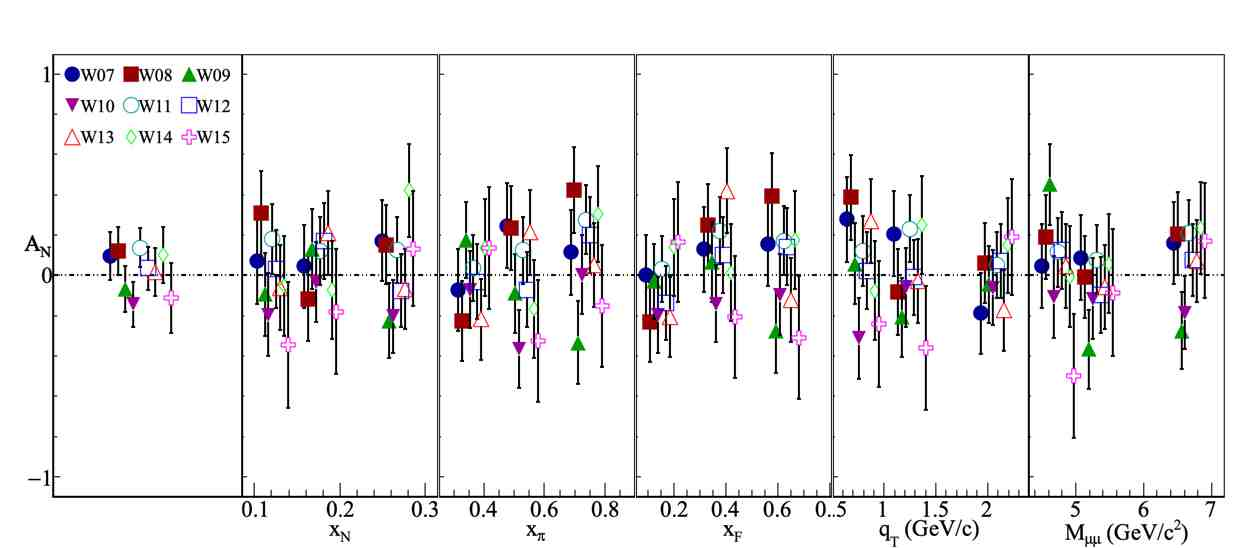
\includegraphics[width=\textwidth]{allPhysBinned4Targ}
    \caption{A$_{\mathrm{N}}$ determined for each period}
    \label{fig::allPhysBinned4Targ}
  \end{center}
\end{figure}

\noindent
By eye the asymmetry fluctuations appear to be statistically compatible.  To
quantify the compatibility of the asymmetries between the periods, a pull
distribution is formed.  The pull value is defined as

\begin{equation}
  \label{eq::pull}
  \Delta\mathrm{A}_i =
  \frac{
    \mathrm{A}_i - \langle \mathrm{A} \rangle
  }{
    \sqrt{
      \sigma^2_{\mathrm{A}_i} - \sigma^2_{\langle \mathrm{A} \rangle}
    }
  },
\end{equation}

\noindent
and is determined for each period and kinematic bin.  There are therefore
3(number of bins)x5(number of kinematics)x9(number of periods) = 135 entries in
the pull distribution. This distribution is shown in Fig.~\ref{fig::pull4Targ}
along with a Gaussian fit.  If the asymmetries all come from the same parent
distribution then due to the central limit theorem the pull distribution will be
a Gaussian distribution with zero mean and unit variance.  The discrepancy of
the pull distribution from a standard Gaussian distribution is used to determine
a systematic error as

\begin{equation}
  \label{equ::sysErrorPull}
  \frac{\sigma_{\mathrm{systematic}}}{\sigma_{\mathrm{statistical}}} =
  \sqrt{|\sigma^2_{\mathrm{pull}} - 1|} + \frac{\mu_{\mathrm{pull}}}{2}.
\end{equation}

\begin{figure}[h!t]
  \begin{center}
    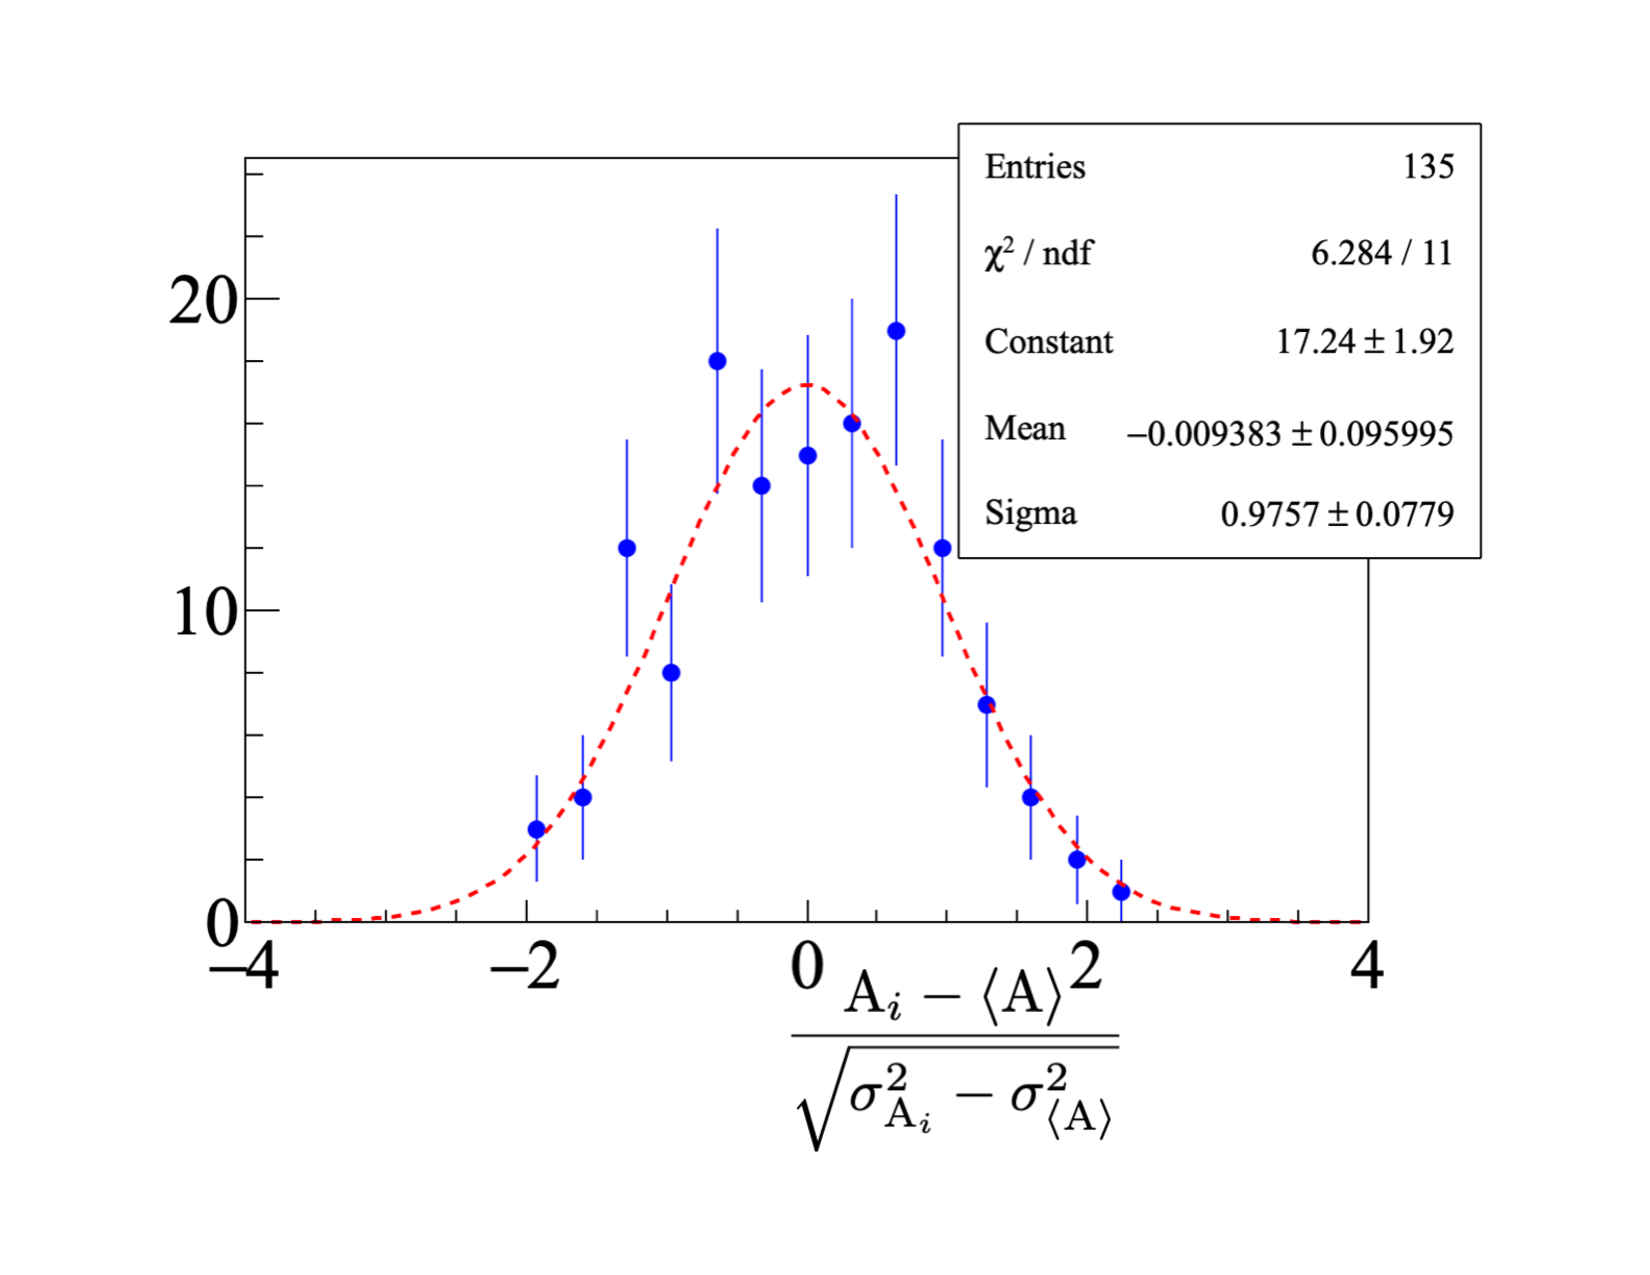
\includegraphics[width=0.8\textwidth, trim=0cm 0cm 0cm 2cm,clip]{pull4Targ}
    \caption{Pull distribution from the two target geometric mean}
    \label{fig::pull4Targ}
  \end{center}
\end{figure}

\noindent
As the asymmetries in different kinematic bins are formed using the same data
set the asymmetries between kinematics are correlated.  For this reason an
uncorrelated pull distribution is also formed for each physics kinematic bin and
also compared with a standard Gaussian distribution.  These distributions are
shown in Fig.~\ref{fig::allPhysPulls4Targ} and the results of the Gaussian fit
are shown in Fig.~\ref{fig::allPhysPulls4Targ_fit}.  For these uncorrelated pull
distributions there are now only 3(number of bins)x9(number of periods) = 27
entries in each kinetically binned pull distributions and only 9(number of
periods) bins in the integrated pull distribution.

\begin{figure}[h!t]
  \begin{center}
    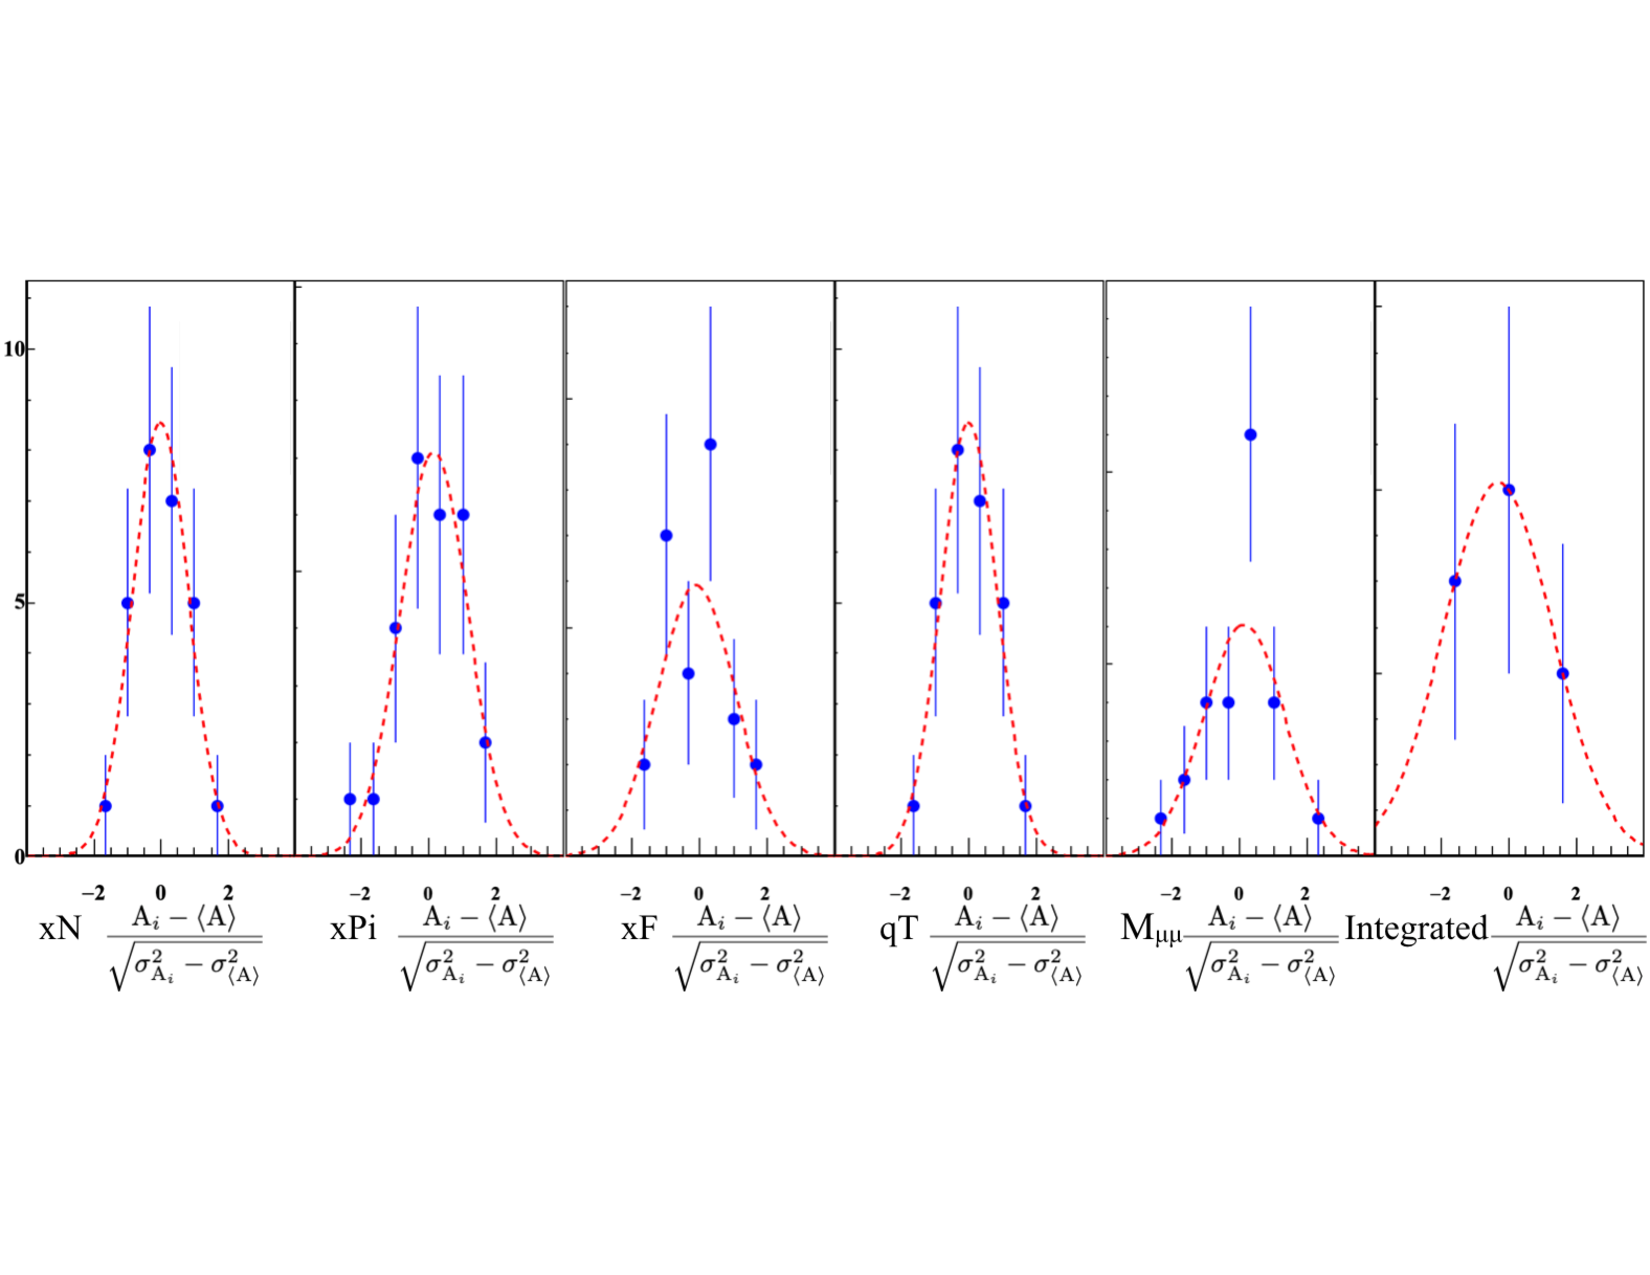
\includegraphics[width=\textwidth, trim=0cm 5cm 0cm 4cm,
      clip]{allPhysPulls4Targ}
    \caption{Uncorrelated pull distributions}
    \label{fig::allPhysPulls4Targ}
  \end{center}
\end{figure}

\begin{figure}[h!t]
  \begin{center}
    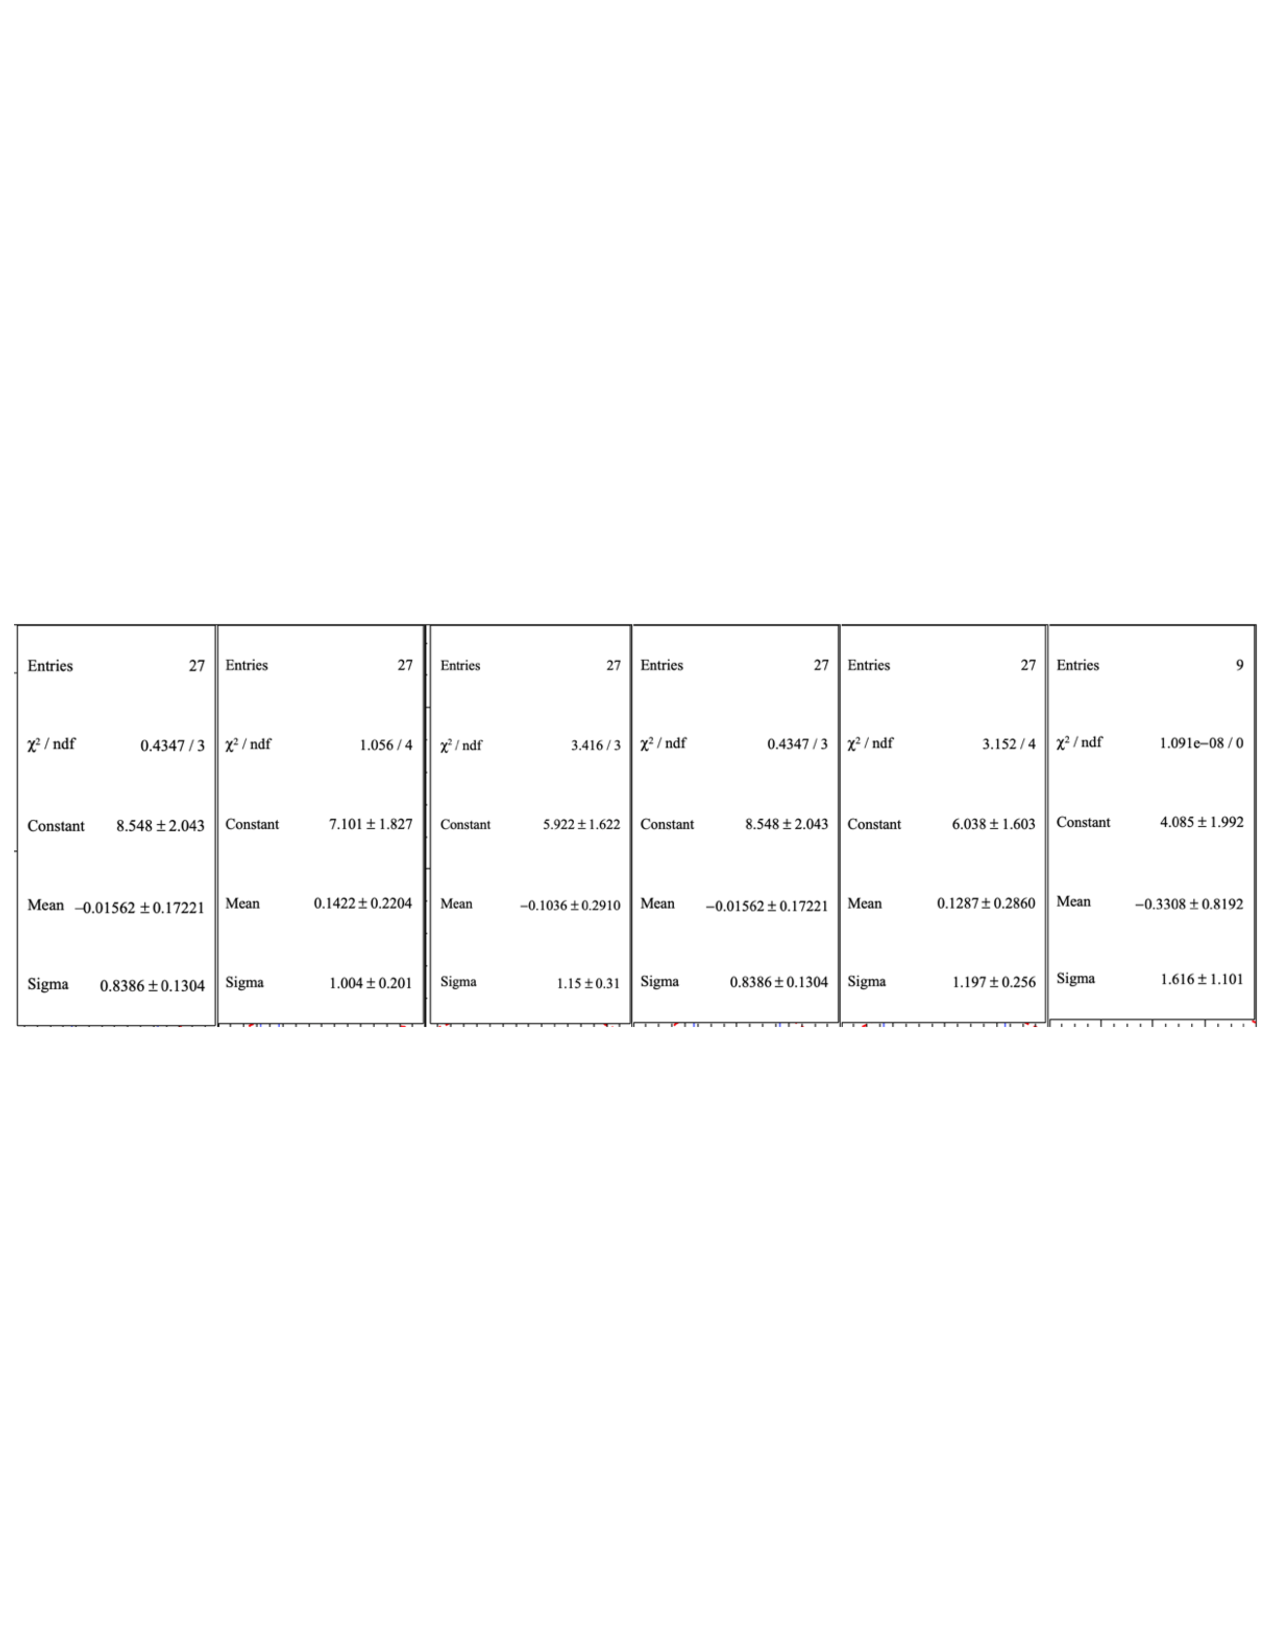
\includegraphics[width=\textwidth, trim=0.2cm 9cm 0.2cm 10cm,
      clip]{allPhysPulls4Targ_fit}
    \caption{Results of Gaussian fit for the uncorrelated pull distributions}
    \label{fig::allPhysPulls4Targ_fit}
  \end{center}
\end{figure}

Even though the Gaussian fits did not give exactly as standard Gaussian, the fit
parameters well compatible with a standard Gaussian within the errors of the
fit.  Therefore no systematic error was assigned due to incompatibility of the
periods.

\subsection{False Asymmetries}
\subsubsection{Acceptance From False Asymmetries}
As was pointed out in Sec.~\ref{sec::GeoMean} and
Sec.~\ref{sec::TwoTargGeoMean}, the asymmetry measurement assumes the acceptance
does not change with time and therefore the acceptance ratios
Eq.~\ref{equ::accGeoMean} and Eq.~\ref{equ::acc4TargGeoMean} are unitary.  Any
deviation from a unitary acceptance ratio is estimated with a false asymmetry
and the errors are included as systematic errors.  To determine if acceptance
does change with time, a false asymmetry is calculated where the only way the
false asymmetry could be non-zero is if acceptance changes with time.  This
false asymmetry for the two target geometric mean is

\begin{equation}
  \label{eqn::falseAcc}
  \begin{split}
    A_{\mathrm{N,False}} &= 
    \frac{1}{\mathrm{P}}
    \frac{
      \sqrt[4]{
        N_{\mathrm{up,Right}}^{\uparrow}N_{\mathrm{up, Left}}^{\downarrow}
        N_{\mathrm{down,Left}}^{\uparrow}N_{\mathrm{down, Right}}^{\downarrow}
      } -
      \sqrt[4]{
        N_{\mathrm{up,Left}}^{\uparrow}N_{\mathrm{up, Right}}^{\downarrow}
        N_{\mathrm{down,Right}}^{\uparrow}N_{\mathrm{down, Left}}^{\downarrow}
      }
    }{
      \sqrt[4]{
        N_{\mathrm{up,Right}}^{\uparrow}N_{\mathrm{up, Left}}^{\downarrow}
        N_{\mathrm{down,Left}}^{\uparrow}N_{\mathrm{down, Right}}^{\downarrow}
      } +
      \sqrt[4]{
        N_{\mathrm{up,Left}}^{\uparrow}N_{\mathrm{up, Right}}^{\downarrow}
        N_{\mathrm{down,Right}}^{\uparrow}N_{\mathrm{down, Left}}^{\downarrow}
      }
    }\\
    & =
    \frac{1}{\mathrm{P}}
    \frac{
      \alpha \sqrt[4]{\sigma_{Right}\sigma_{Left}\sigma_{Left}\sigma_{Right}} -
      \sqrt[4]{\sigma_{Left}\sigma_{Right}\sigma_{Right}\sigma_{Left}}
    }{
      \alpha \sqrt[4]{\sigma_{Right}\sigma_{Left}\sigma_{Left}\sigma_{Right}} +
      \sqrt[4]{\sigma_{Left}\sigma_{Right}\sigma_{Right}\sigma_{Left}}
    }
  \end{split}
\end{equation}

\begin{equation}
  \label{equ::alphaAsym}
  = \frac{1}{\mathrm{P}}
  \frac{
    \alpha - 1     
  }{
    \alpha + 1
  },
\end{equation}

\noindent
where $\alpha$ is an acceptance ratio and is defined as

\begin{equation}
  \frac{
    \sqrt[4]{
      \mathrm{a}^{\uparrow}_{\mathrm{up,Saleve}}
      \mathrm{a}^{\downarrow}_{\mathrm{up,Saleve}}
      \mathrm{a}^{\uparrow}_{\mathrm{down,Jura}}
      \mathrm{a}^{\downarrow}_{\mathrm{down,Jura}}}
  }{
    \sqrt[4]{
      \mathrm{a}^{\uparrow}_{\mathrm{up,Jura}}
      \mathrm{a}^{\downarrow}_{\mathrm{up,Jura}}
      \mathrm{a}^{\uparrow}_{\mathrm{down,Saleve}}
      \mathrm{a}^{\downarrow}_{\mathrm{down,Saleve}}}
  }.
\end{equation}

\noindent
The false asymmetry, Eq.~\ref{eqn::falseAcc}, can be simplified as

\begin{equation}
  A_{\mathrm{N,False}} = 
  \frac{1}{\mathrm{P}}
  \frac{
    \sqrt[4]{
      N_{\mathrm{up, Saleve}}
      N_{\mathrm{down, Jura}}
    } -
    \sqrt[4]{
      N_{\mathrm{up, Jura}}
      N_{\mathrm{down, Saleve}}
    }
  }{
    \sqrt[4]{
      N_{\mathrm{up, Saleve}}
      N_{\mathrm{down, Jura}}
    } +
    \sqrt[4]{
      N_{\mathrm{up, Jura}}
      N_{\mathrm{down, Saleve}}
    }
  }.
\end{equation}

\noindent
That is A$_{\mathrm{N,false}}$ is the normalized difference of counts from each
target cell assuming the upstream target is always polarized down and the
downstream target is always polarized up.  Given that the polarization flips for
both upstream and downstream target cells, A$_{\mathrm{N,false}}$ is an
asymmetry where physical effects cancel out.  The kinematic dependencies of the
false asymmetry are shown in Fig.~\ref{fig::falseAacc} and the kinematic
dependencies of the acceptance ratio, $\alpha$, are shown in
Fig.~\ref{fig::alpha}.

\begin{figure}[h!t]
  \begin{center}
    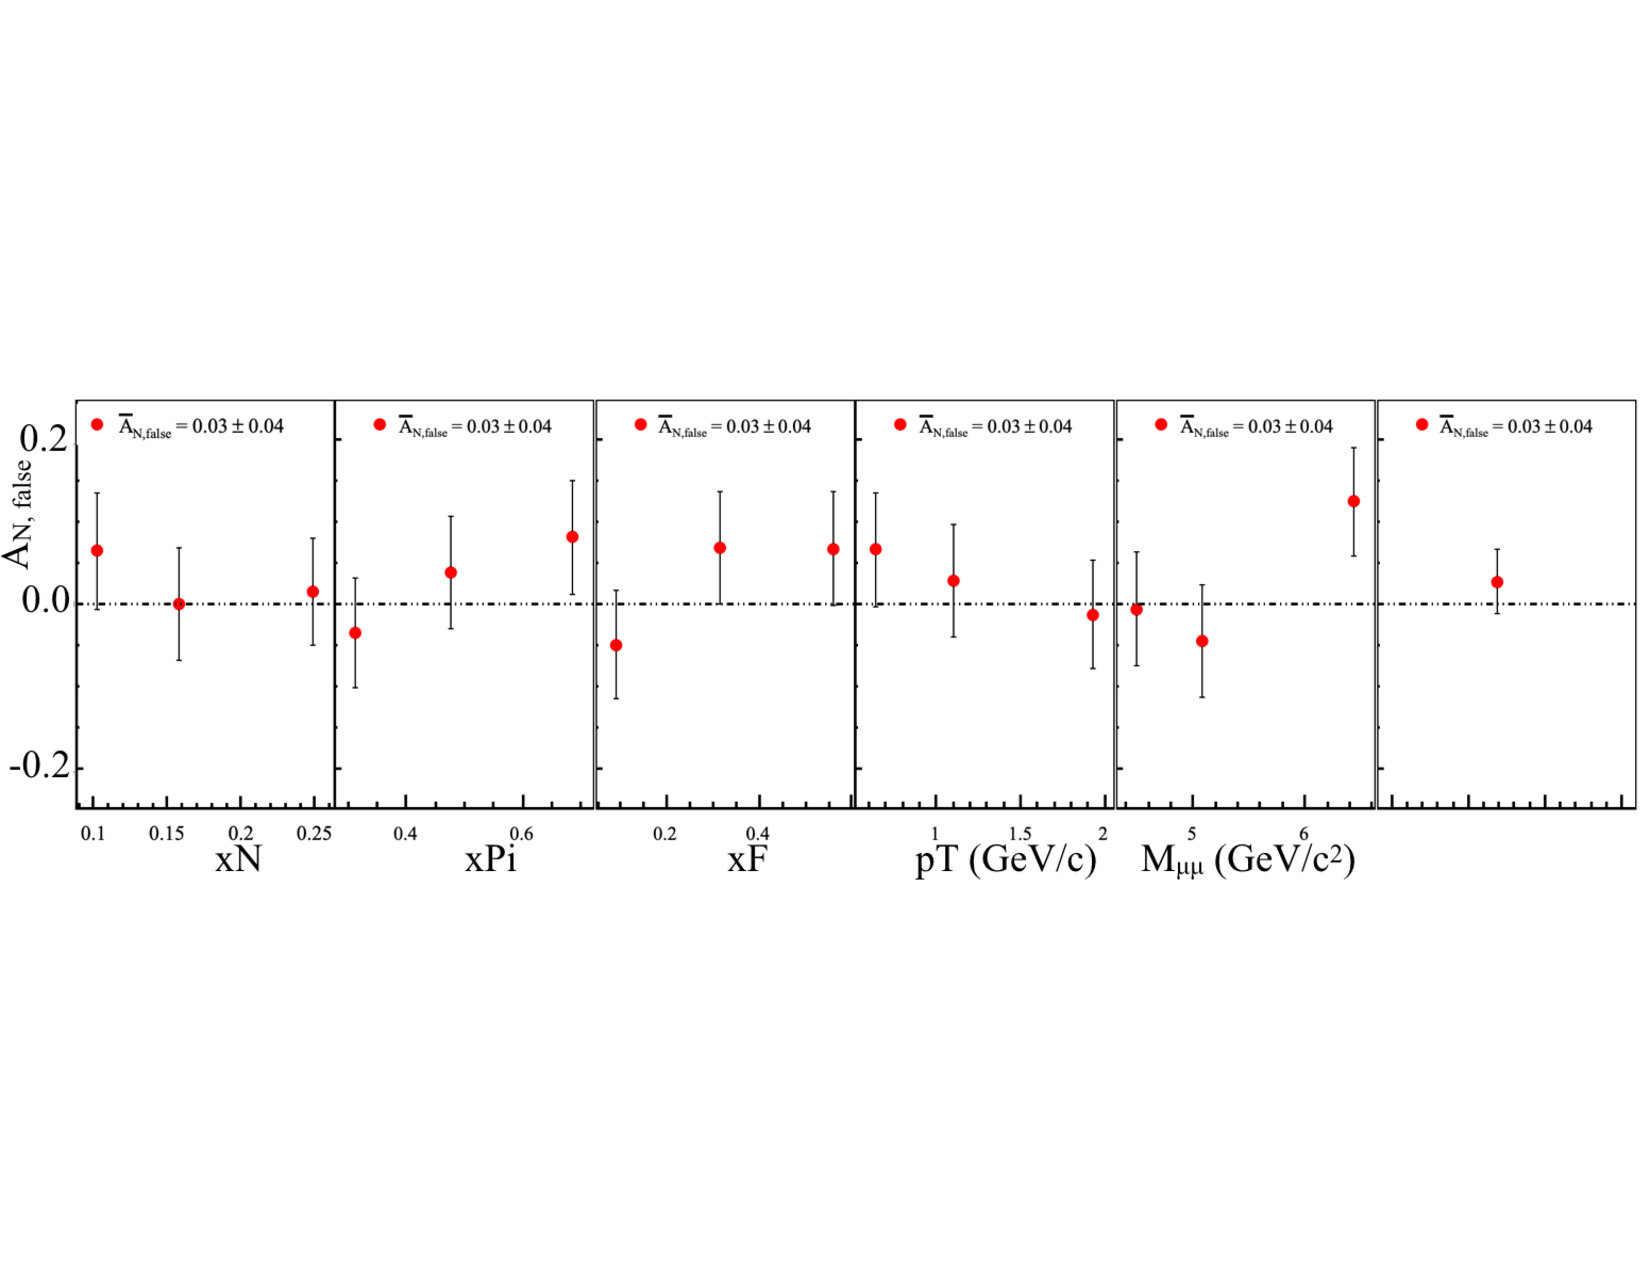
\includegraphics[width=\textwidth, trim=0cm 6.5cm 0cm 6.5cm,
      clip]{falseAacc}
    \caption{False asymmetry to estimate fluctuations in acceptance in time}
    \label{fig::falseAacc}
  \end{center}
\end{figure}

\begin{figure}[h!t]
  \begin{center}
    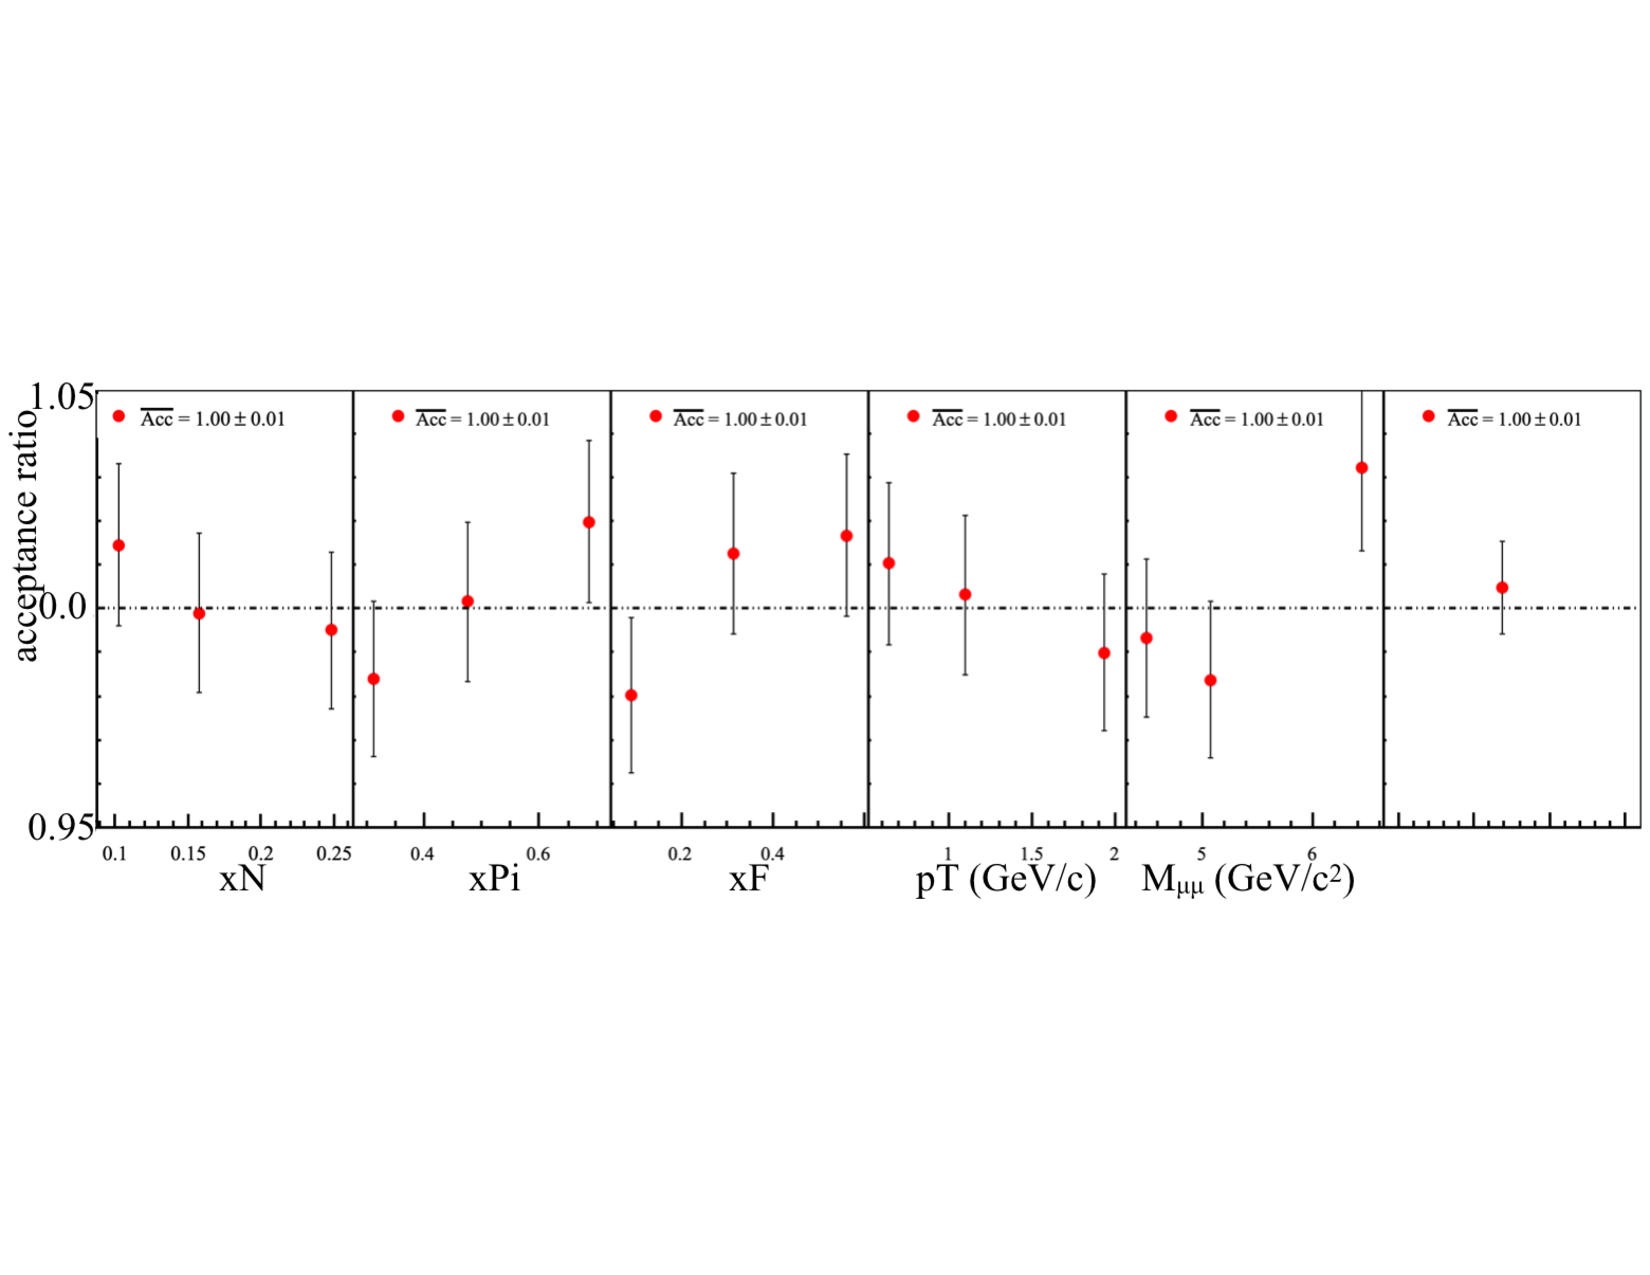
\includegraphics[width=\textwidth, trim=0cm 6cm 0cm 6cm,
      clip]{alpha4Targ}
    \caption{Acceptance ratio used to determine the systematic effects from
      acceptance changes in time}
    \label{fig::alpha}
  \end{center}
\end{figure}

While $\alpha$ is an acceptance ratio it is not the same as the acceptance ratio
in the true asymmetry.  However $\alpha$ is similar to the true acceptance
ratio, $\kappa$, in that $\alpha$ will only be different from unity as a result
of time changes in the spectrometer.  Therefore it is assumed $\alpha$ can be
used as a good estimate of the true acceptance ratio fluctuations.  The
systematic error due to acceptance fluctuations is determined as

\begin{equation}
  \delta\mathrm{A}_{\mathrm{N,systematic}} =
  \frac{1}{P} \Big(\frac{|\alpha-1|}{2} + \delta_{\frac{|\alpha-1|}{2}} \Big),
\end{equation}

\noindent
where this expression is derived in Appendix~\ref{app::sysAcc}.  The kinematic
dependence of the systematic error normalized to the statistical error is shown
in Fig.~\ref{fig::accSysStat}.  The binned average systematic error due to
acceptance is 20\% of the statistical error.

\begin{figure}[h!t]
  \begin{center}
    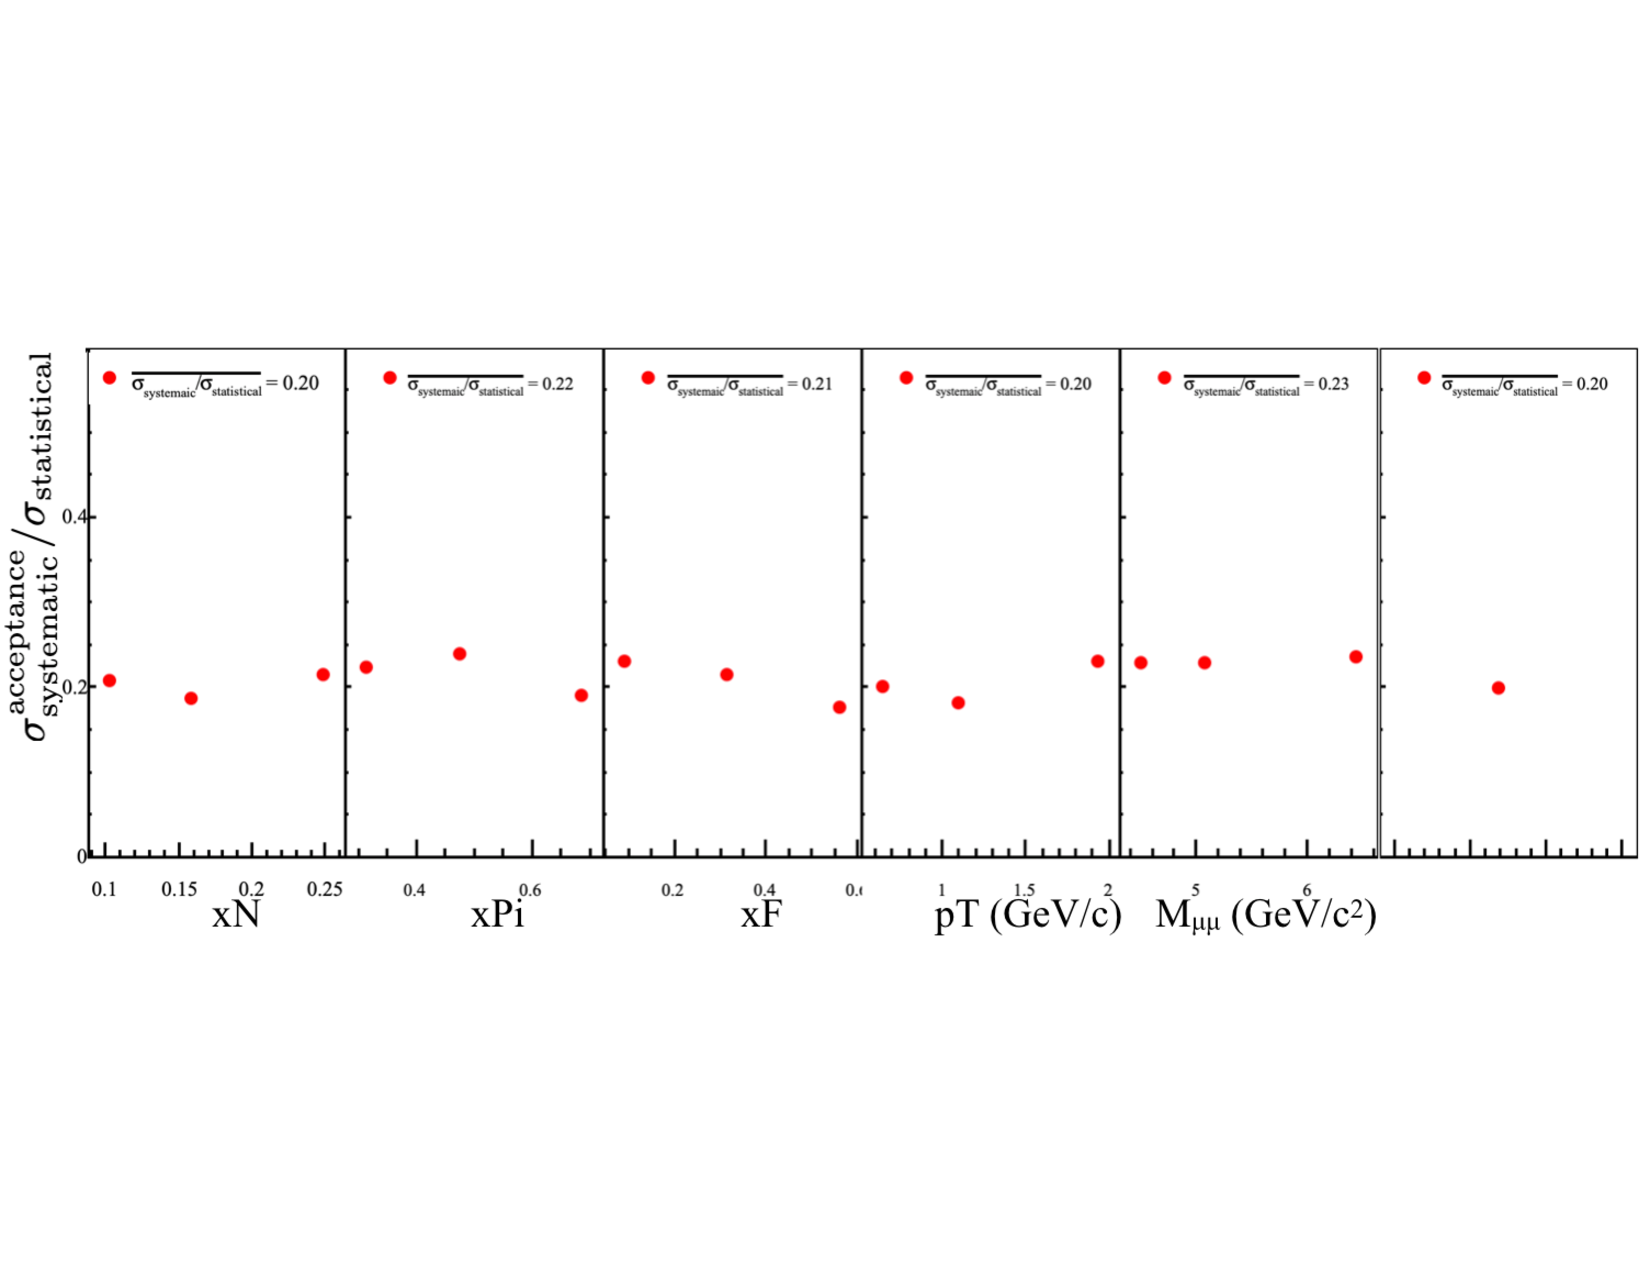
\includegraphics[width=\textwidth, trim=0cm 5cm 0cm 5cm,
      clip]{accSysStat}
    \caption{Systematic error due to acceptance effects}
    \label{fig::accSysStat}
  \end{center}
\end{figure}

\subsection{Further False Asymmetry Effects}
Although the list of systematic effects specifically studied is quite exhaustive
there is always the potential for other systematic effects not considered.
Studies of the changes in time from additional false asymmetries were performed
in an attempt to taken into account all other systematic effects.  All false
asymmetries considered must be constructed in such a way that the physical
process of interest cancels out.  A false asymmetry could therefore only be
non-zero from acceptance effects, luminosity or some other reason not
considered.  The additional false asymmetries constructed are made in a way that
luminosity effects canceled out and acceptance effects were approximately
constant.  With these assumptions pull values from Eq.~\ref{eq::pull} should be
distributed as a standard Gaussian distribution.  Any deviation from a standard
Gaussian is conservatively taken as a systematic effect from some unknown cause.
The additional studied false asymmetries are summarized in the following
enumerated list.

\begin{enumerate}
  \label{tab::additionalFA}

\item A false asymmetry similar to Eq.~\ref{eqn::falseAcc} but with the upstream
  left and right counts flipped defined as
  
  \begin{equation}
    \label{eqn::additionalfalseAsym}
    \frac{1}{\mathrm{P}}
    \frac{
      \sqrt[4]{
        N_{\mathrm{up,Left}}^{\uparrow}N_{\mathrm{up,Right}}^{\downarrow}
        N_{\mathrm{down,Left}}^{\uparrow}N_{\mathrm{down,Right}}^{\downarrow}
      } -
      \sqrt[4]{
        N_{\mathrm{up,Right}}^{\uparrow}N_{\mathrm{up,Left}}^{\downarrow}
        N_{\mathrm{down,Right}}^{\uparrow}N_{\mathrm{down, Left}}^{\downarrow}
      }
    }{
      \sqrt[4]{
        N_{\mathrm{up,Left}}^{\uparrow}N_{\mathrm{up,Right}}^{\downarrow}
        N_{\mathrm{down,Left}}^{\uparrow}N_{\mathrm{down, Right}}^{\downarrow}
      } +
      \sqrt[4]{
        N_{\mathrm{up,Right}}^{\uparrow}N_{\mathrm{up,Left}}^{\downarrow}
        N_{\mathrm{down,Right}}^{\uparrow}N_{\mathrm{down, Left}}^{\downarrow}
      }
    }.
  \end{equation}
  This false asymmetry can be thought of as measuring the normalized counts on
  the Jura side minus the Saleve side.  The period weighted average results of
  this false asymmetry are shown in Fig.~\ref{fig::fa2TargJuraSaleve} and as can
  be seen there is the asymmetry is systematically less than zero by more than a
  standard deviation.  The uncorrelated pull distributions from this false
  asymmetry are shown in Fig.~\ref{fig::fa2TargJSPulls} and the corresponding
  Gaussian fit results are shown in Fig.~\ref{fig::fa2TargJSPulls_fit}.  Due to
  the fact that there are less entries in these pull distributions the Gaussian
  fit results are not necessarily that good.  In an attempt to correct for this
  and to take into account the fit errors, a weighted average of the mean and
  standard deviation are made, as in Eq.~\ref{equ::wAvg}, using weights as the
  inverse fit variances.  The resulting systematic error is again determined as
  in Eq.~\ref{equ::sysErrorPull} using the weighted mean and weighted standard
  deviation.

  \begin{figure}[h!t]
    \centering
    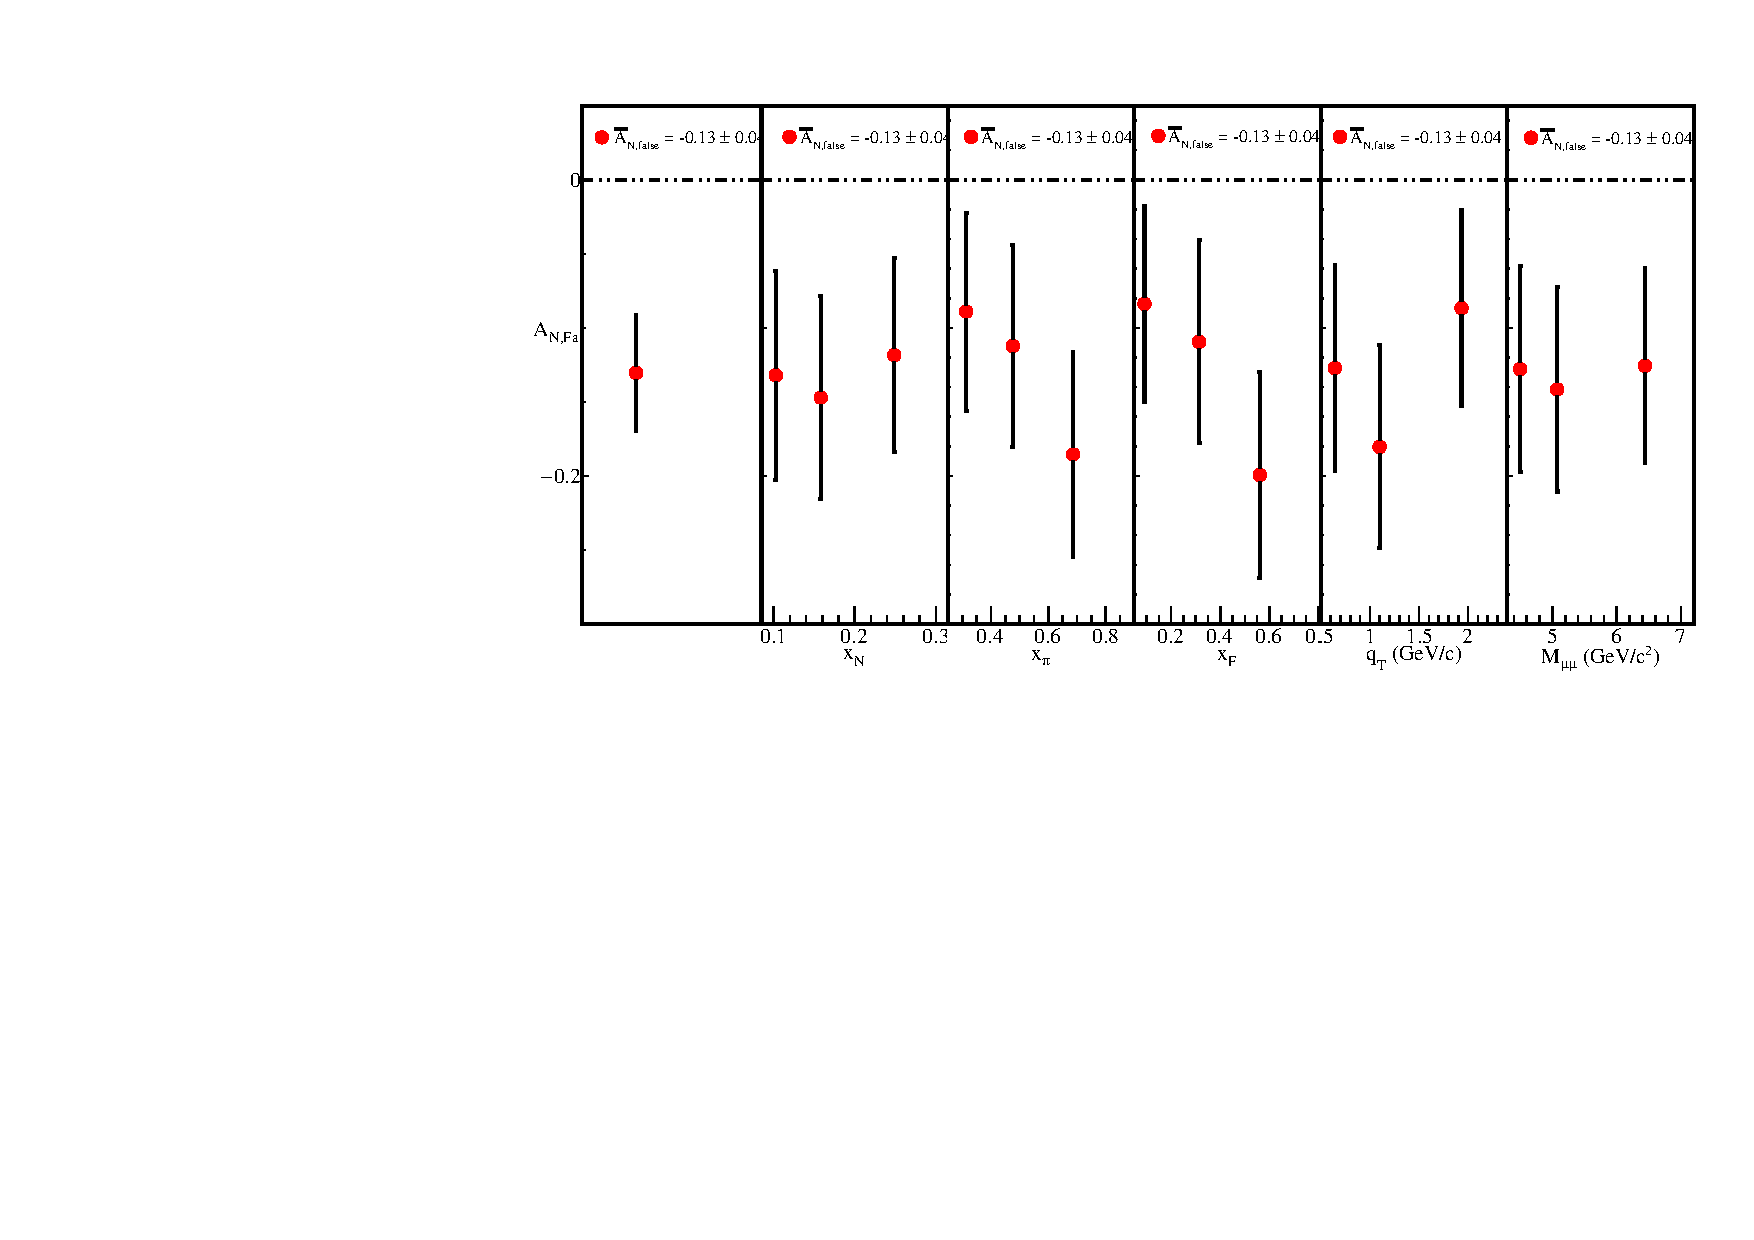
\includegraphics[width=\textwidth]{fa2TargJuraSaleve}
    \caption{Two target geomean false asymmetry.  This is non-zero due to
      acceptance effects}
    \label{fig::fa2TargJuraSaleve}
  \end{figure}
  
  \begin{figure}[h!t]
    \centering
    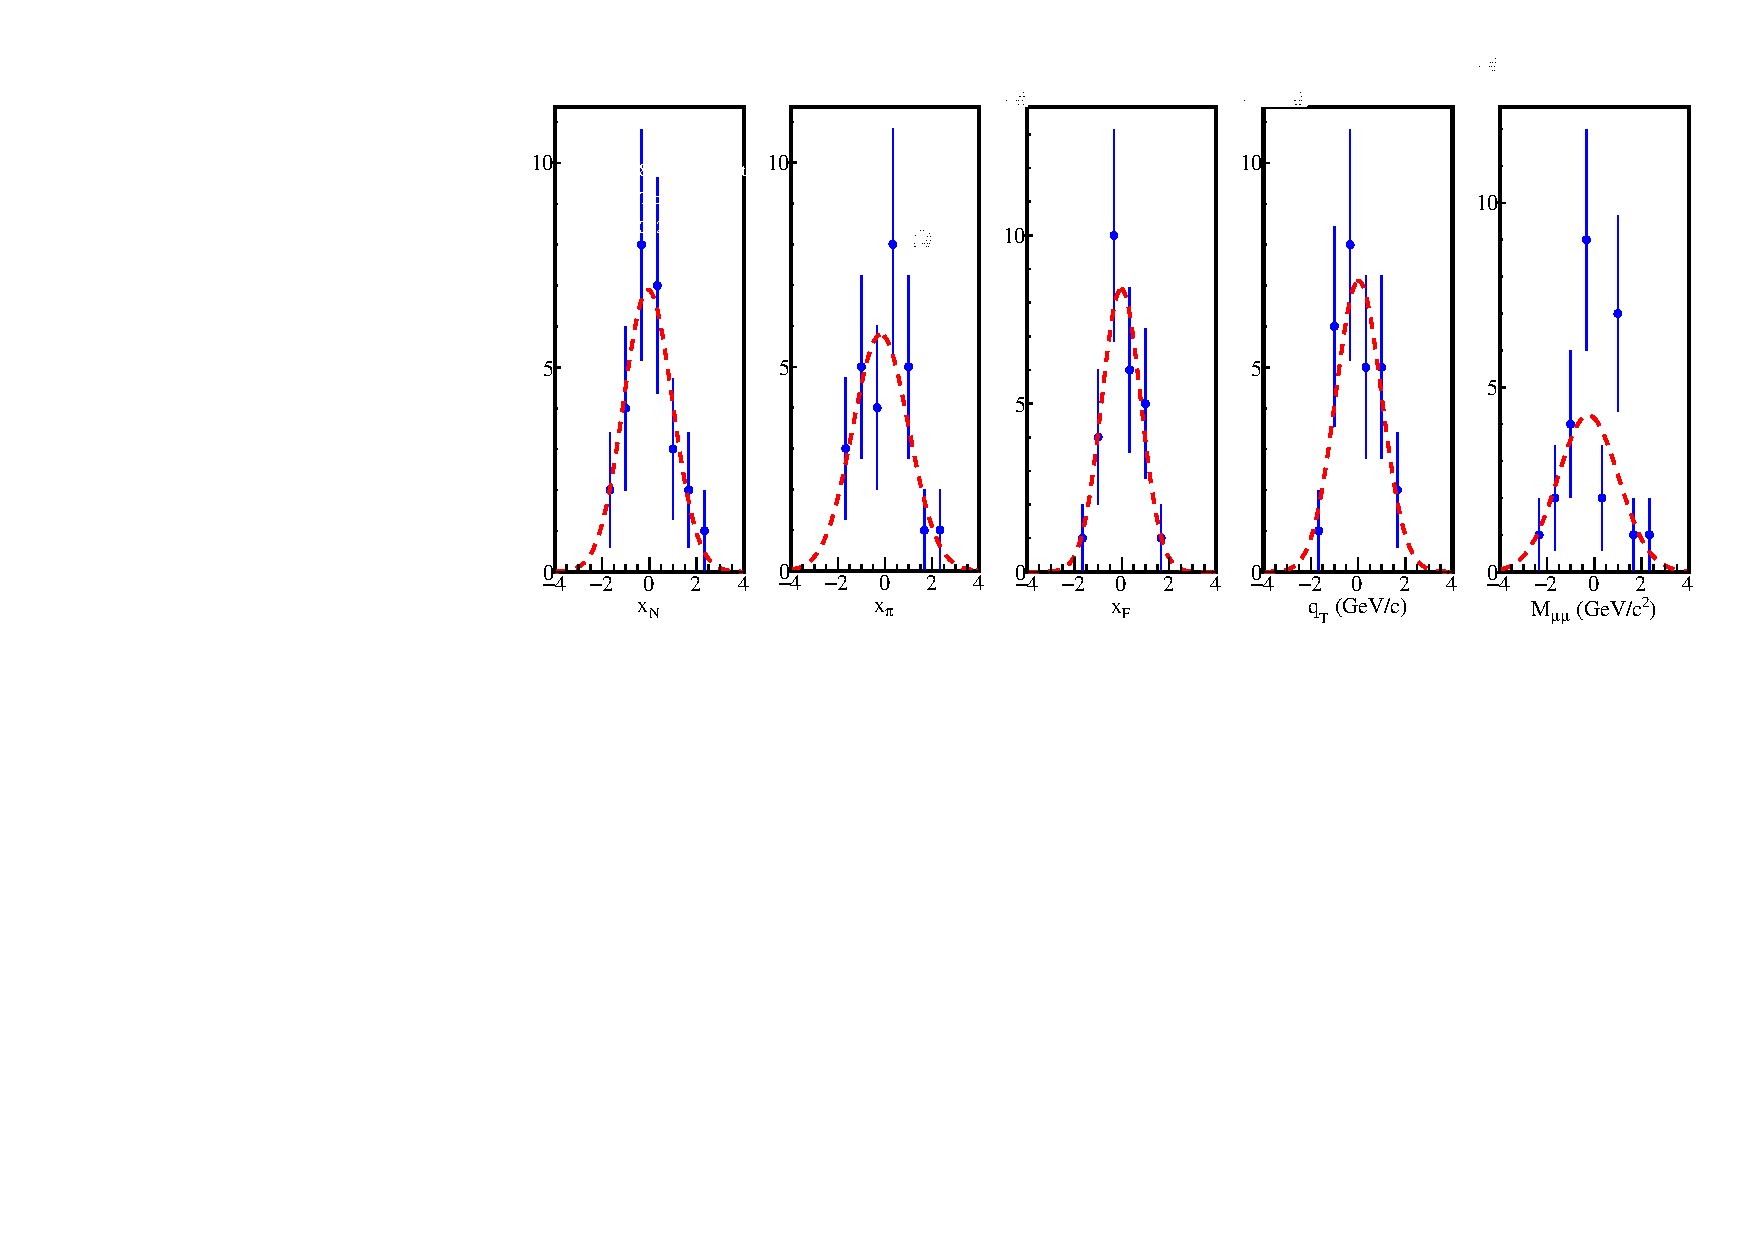
\includegraphics[width=\textwidth]{fa2TargJSPulls}
    \caption{Uncorrelated pulls of the two target geomean false asymmetry}
    \label{fig::fa2TargJSPulls}
  \end{figure}
  
  \begin{figure}[h!t]
    \centering
    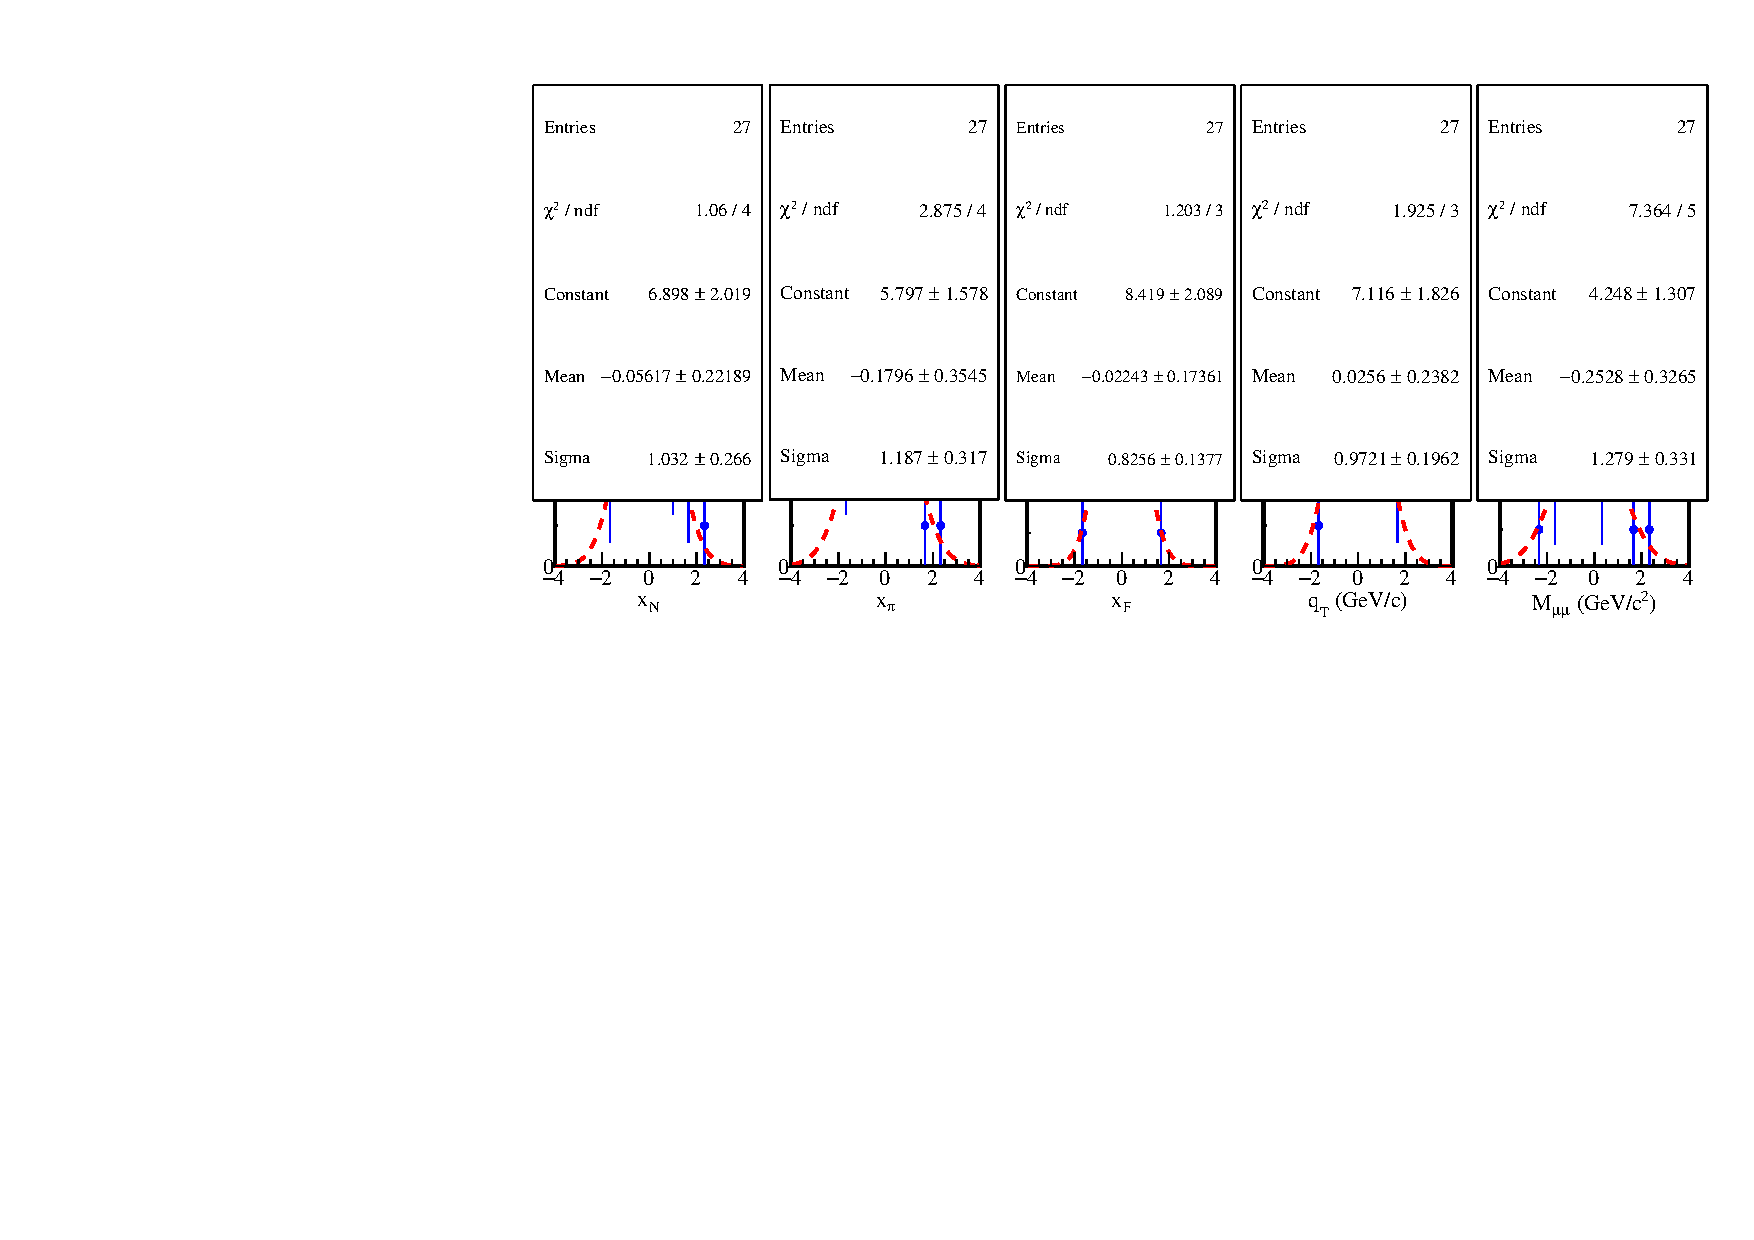
\includegraphics[width=\textwidth, trim=0cm 2.15cm 0cm 0cm, clip]
                    {fa2TargJSPulls_fit}
                    \caption{Gaussian git results for the uncorrelated two
                      target false geomean pulls}
                    \label{fig::fa2TargJSPulls_fit}
  \end{figure}

\item A false asymmetries using only the information from the upstream or the
  downstream target defined as

  \begin{equation}
    \label{eqn::falseANgeomean}
    \frac{1}{\mathrm{P}} \frac{\sqrt{N_{\mathrm{up(down)stream,
            Left}}^{\uparrow}N_{\mathrm{up(down)stream, Right}}^{\downarrow}} -
      \sqrt{N_{\mathrm{up(down)stream,
            Right}}^{\uparrow}N_{\mathrm{up(down)stream, Left}}^{\downarrow}}
    }{\sqrt{N_{\mathrm{up(down)stream,
            Left}}^{\uparrow}N_{\mathrm{up(down)stream, Right}}^{\downarrow}} +
      \sqrt{N_{\mathrm{up(down)stream,
            Right}}^{\uparrow}N_{\mathrm{up(down)stream, Left}}^{\downarrow}} }.
  \end{equation}
  This false asymmetry can also be thought of as measuring the normalized counts
  on the Jura side minus the Saleve side but for each target individually.  Both
  this false asymmetry and the previous false asymmetry can be written as
  Eq.~\ref{equ::alphaAsym} where $\alpha$ will be an acceptance ratio of
  Jura/Saleve.  As the Jura/Saleve acceptance ratio is expected to be the same
  for the upstream and downstream targets, any difference between the two false
  asymmetries must be due to other reasons.  A by period comparison between the
  upstream and downstream target is shown in Fig.~\ref{fig::alphaAsymPeriod} and
  as can be seen there are difference by period between the upstream and
  downstream asymmetries.  A combined pull distribution is made using the
  information from both upstream and downstream asymmetries and is shown in
  Fig.~\ref{fig::alphaAsymPull}.  As with the previous false asymmetry, lack of
  data leads to the same problems with fit and therefore the same weighting
  method is used to determine a systematic error.

  \begin{figure}[h!t]
    \centering
    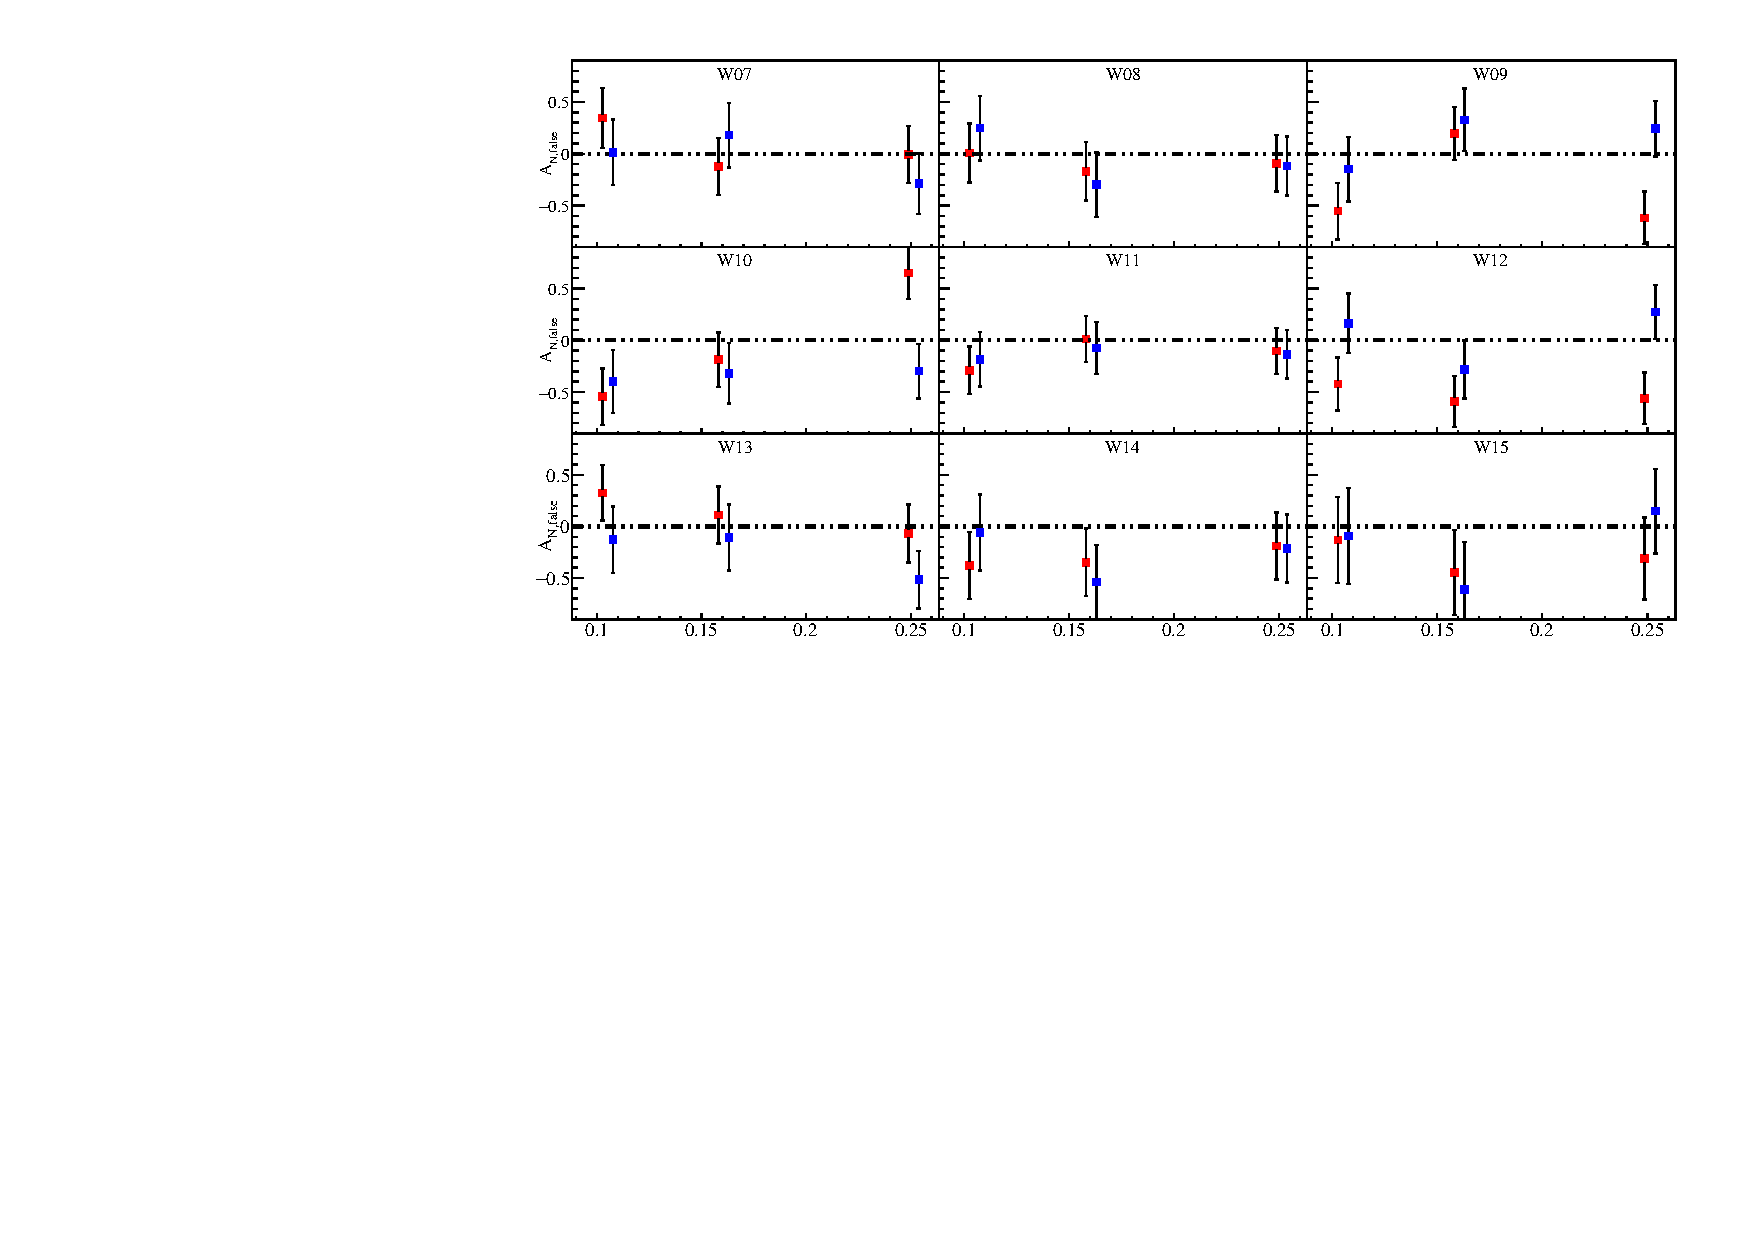
\includegraphics[width=\textwidth]{alphaAsymPeriod}
    \caption{One target false asymmetries for the upstream target (red) and the
      downstream target (blue), as a function of x$_{\mathrm{N}}$.  Each graph
      is from a different period in time.}
    \label{fig::alphaAsymPeriod}
  \end{figure}

  \begin{figure}[h!t]
    \centering
    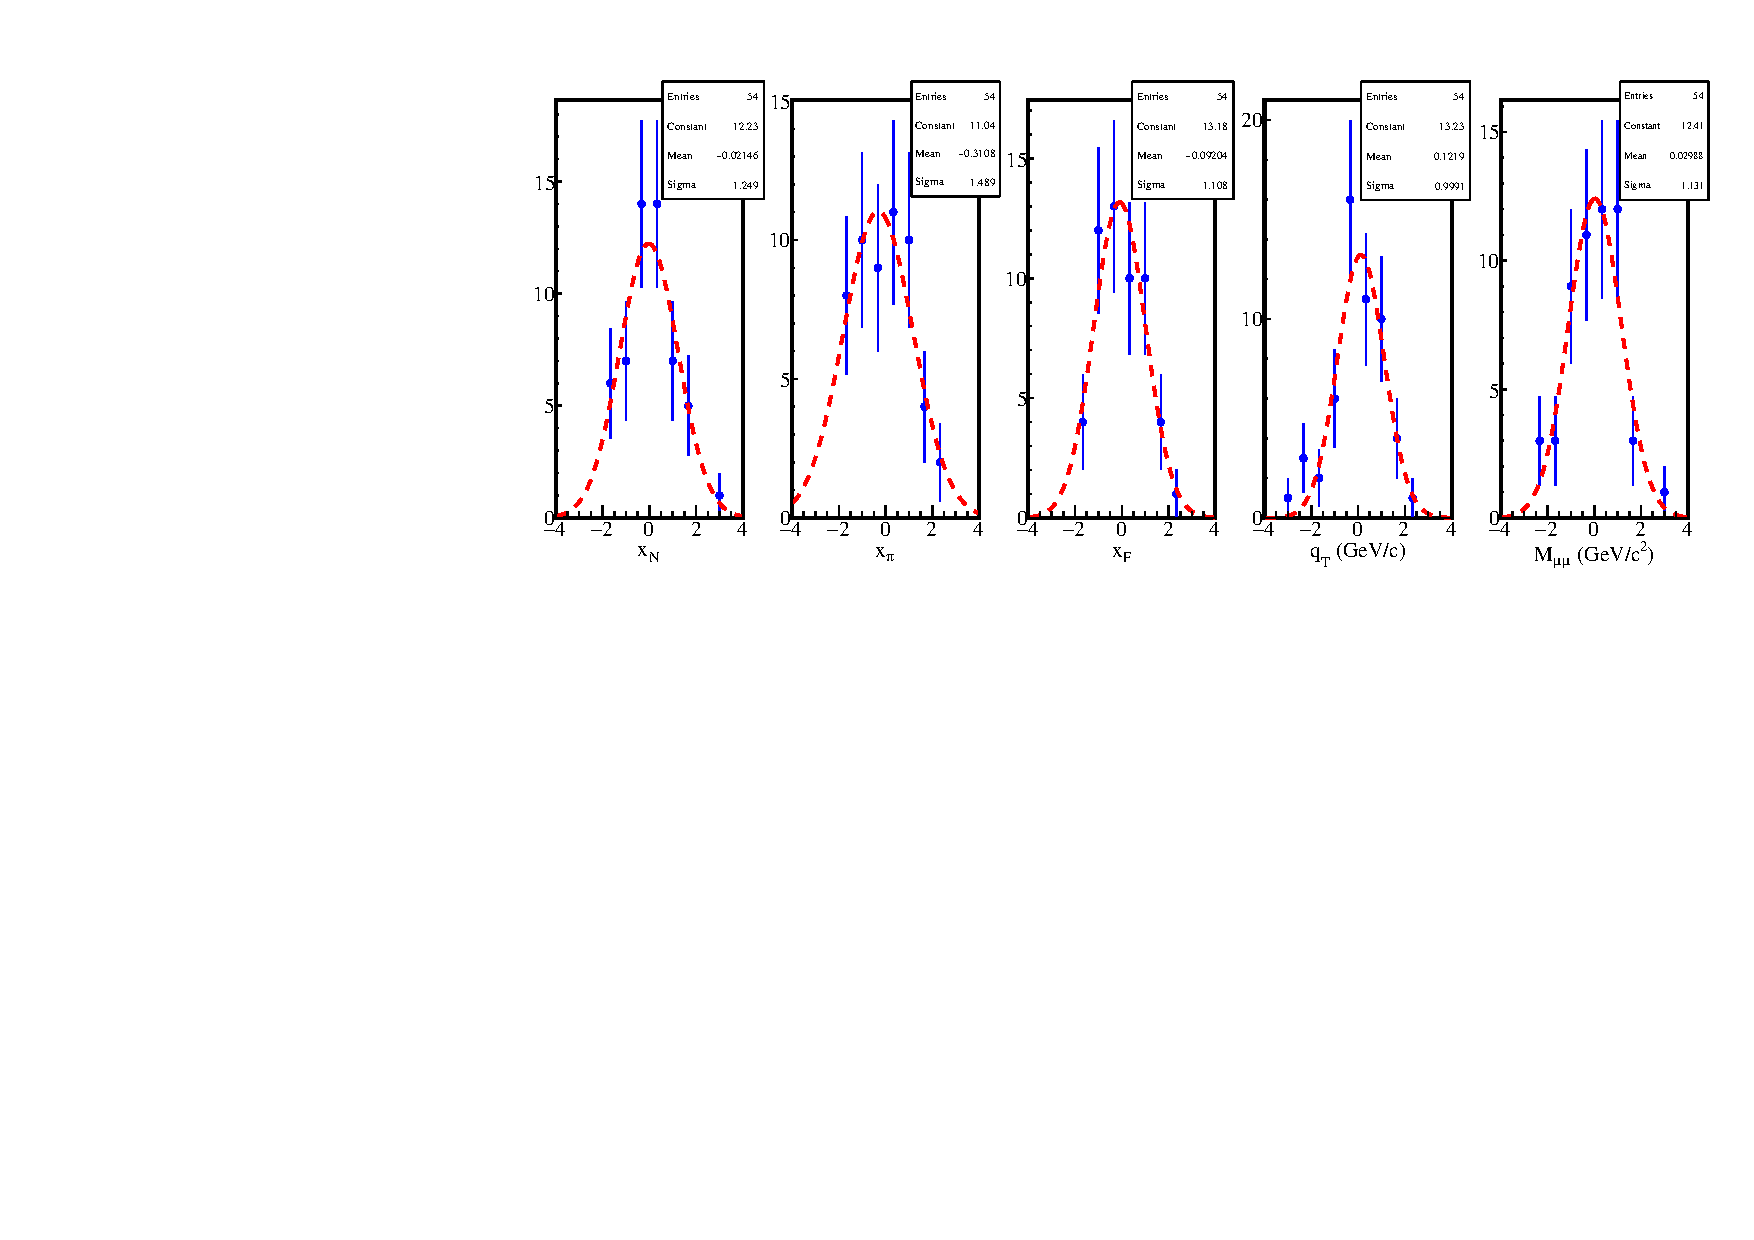
\includegraphics[width=\textwidth]{alphaAsymPull}
    \caption{Pull values from one target geomean false asymmetries.  Both
      upstream and downstream values are used to make this pull}
    \label{fig::alphaAsymPull}
  \end{figure}

\item Finally the same false asymmetry used to determine the acceptance
  fluctuations, Eq.~\ref{eqn::falseAcc}, is also checked for compatibility and a
  systematic error is determined in the same way as the previous false
  asymmetries.  The pulls are shown in Fig.~\ref{fig::fa2TargPulls} and the
  corresponding fit parameters are shown in Fig.~\ref{fig::fa2TargPulls_fit}.

  \begin{figure}[h!t]
    \centering
    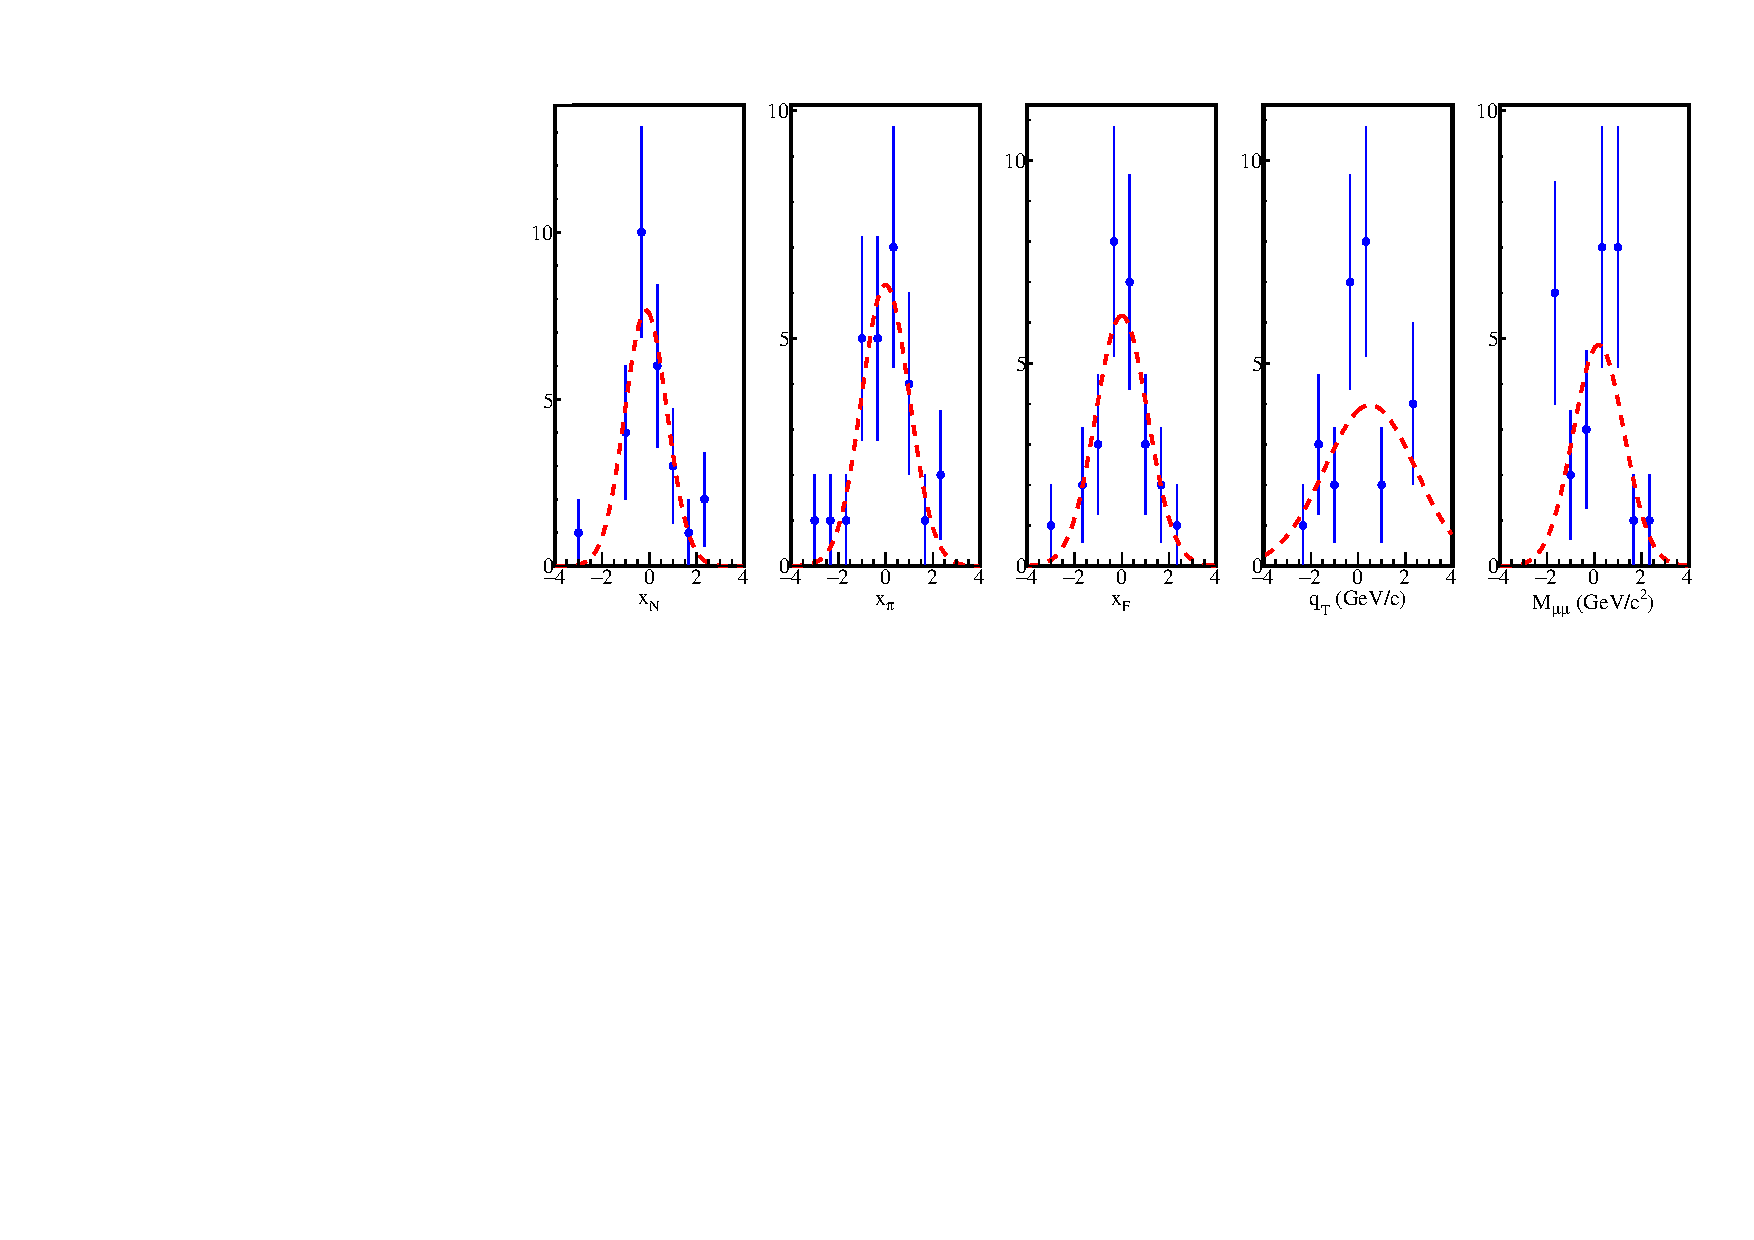
\includegraphics[width=\textwidth]{fa2TargPulls}
    \caption{Pull distribution for a nearly acceptance free two target false
      geomean asymmetry}
    \label{fig::fa2TargPulls}
  \end{figure}
  
  \begin{figure}[h!t]
    \centering
    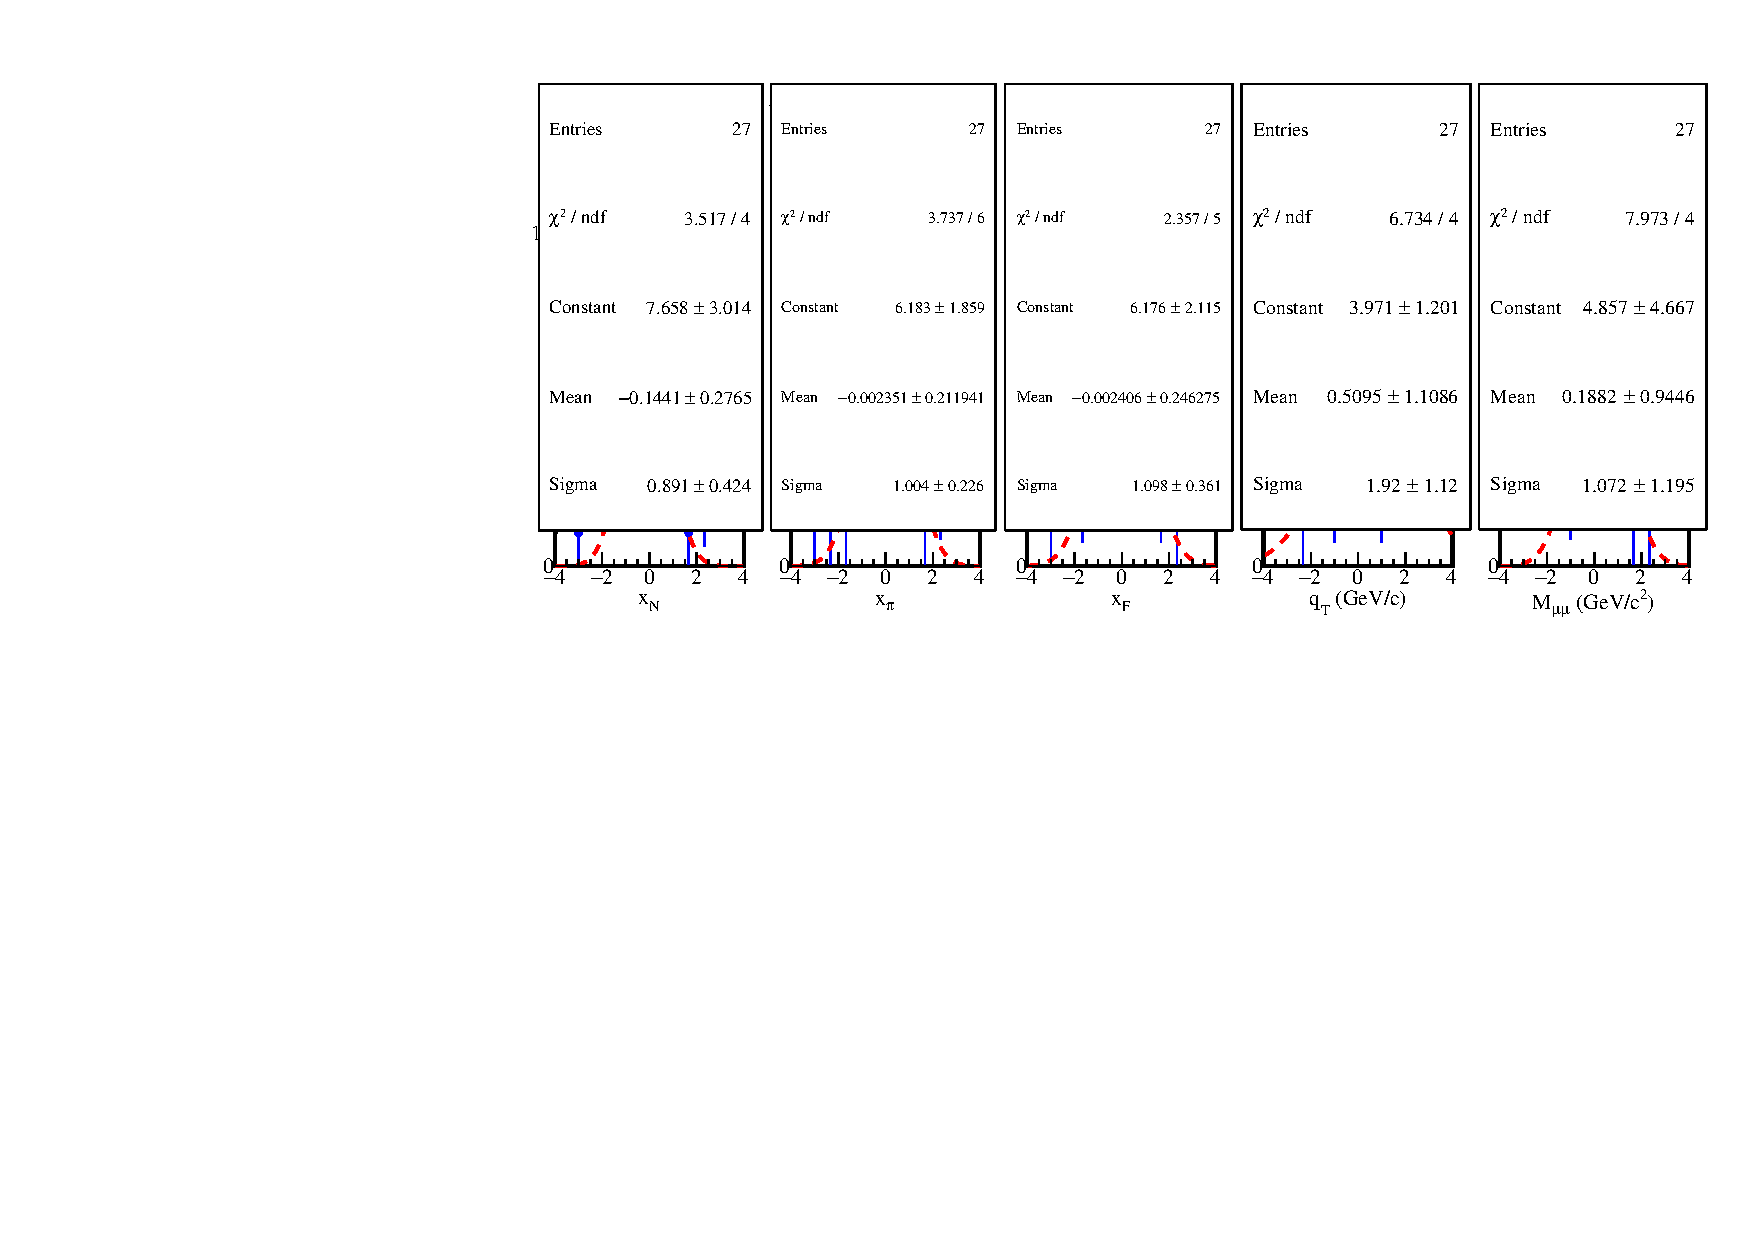
\includegraphics[width=\textwidth,
      trim=0cm 1.65cm 0cm 0cm, clip]{fa2TargPulls_fit}
    \caption{Gaussian fit results for the previous pull
      distributions}
    \label{fig::fa2TargPulls_fit}
  \end{figure}
  
\end{enumerate}

A summary of the systematic error from each false asymmetry is shown in
Tab.~\ref{tab::faSys}

\begin{table}[h!t]
  \centering
  \begin{tabular}{|c|c|}
    \hline Systematic error& \multirow{2}{9em}{$\langle
      \sigma_{\mathrm{systematic}}/\sigma_{\mathrm{statistical}}
      \rangle$}\\ & \\ \hline
    
    Two target Jura-Saleve& 0.26\\ \hline

    Combined one target& 0.5\\ \hline

    Two target acceptance estimation& 0.29\\ \hline
    
  \end{tabular}
  \caption{Summary of systematic error impacts from false asymmetries.  The
    maximum systematic error is chosen as the systematic error.}
  \label{tab::faSys}
\end{table}


\subsection{Left/Right Event Migration}
The spectrometer has finite resolution for any measured quantity and for this
reason events measured as left outgoing could really be events that are right
outgoing and vise versa for measured left outgoing events.  This left-right
miss-identification has the result of diluting spin-dependent effects by
effectively having a sample from an unpolarized target along with the sample
from the polarized target.  Therefore the asymmetry A$_{\mathrm{N}}$ reduces
from left-right miss-identification and this effect is included as a systematic
effect. \par

For this thesis five Monte-Carlo processes were generated corresponding to three
background processes and a spin-independent signal process.  The generated used
was PHTHYIA8 and the data was generated and reconstruction at Blue Waters.  The
background processes simulated were JPsi production, Psi' production and open
charm (OC) production.  Each of these backgrounds can decay into two muons which
results in a background contamination to the Drell-Yan signal.
Table~\ref{tab::MCproduction} gives the parameters used for the Monte-Carlo
studied.

\begin{table}[h!t]
  \centering
  \label{tab::MCproduction}
  \caption{Monte-Carlo settings produced on Blue Waters}
  \begin{tabular}{ |c|c| }
    \hline
    Event generator& PYTHIA8\\
    \hline

    Pion pdf& GRVPI1\\
    \hline

    Proton pdf& NNPDF23\\
    \hline
    
    proton/neutron mixing ratio& 1.96\\
    \hline

    Initial state radiation& on\\
    \hline
    
    Final state radiation& on\\
    \hline
    
    Multiple parton interactions& on\\
    \hline

    Simulated detector efficiencies& uniform\\
    \hline
    
  \end{tabular}
\end{table}

Miss-identification was estimated from the simulated Monte-Carlo data sample
described in Table~\ref{tab::MCproduction} where the sample was made from the
respond of the COMPASS spectrometer to input Drell-Yan events in a similar mass
range.  The same analysis performed on real data was performed on this
Monte-Carlo data to get the angles of interest.  Fig.~\ref{fig::lrMigration}
shows the rate of events identified correctly and incorrectly as a function of
the $\phi_{\mathrm{S}}$.  This plot is made by determining which outgoing
direction the generated events emerged with the outgoing direction the
reconstructed events emerged.

\begin{figure}[h!t]
  \centering
  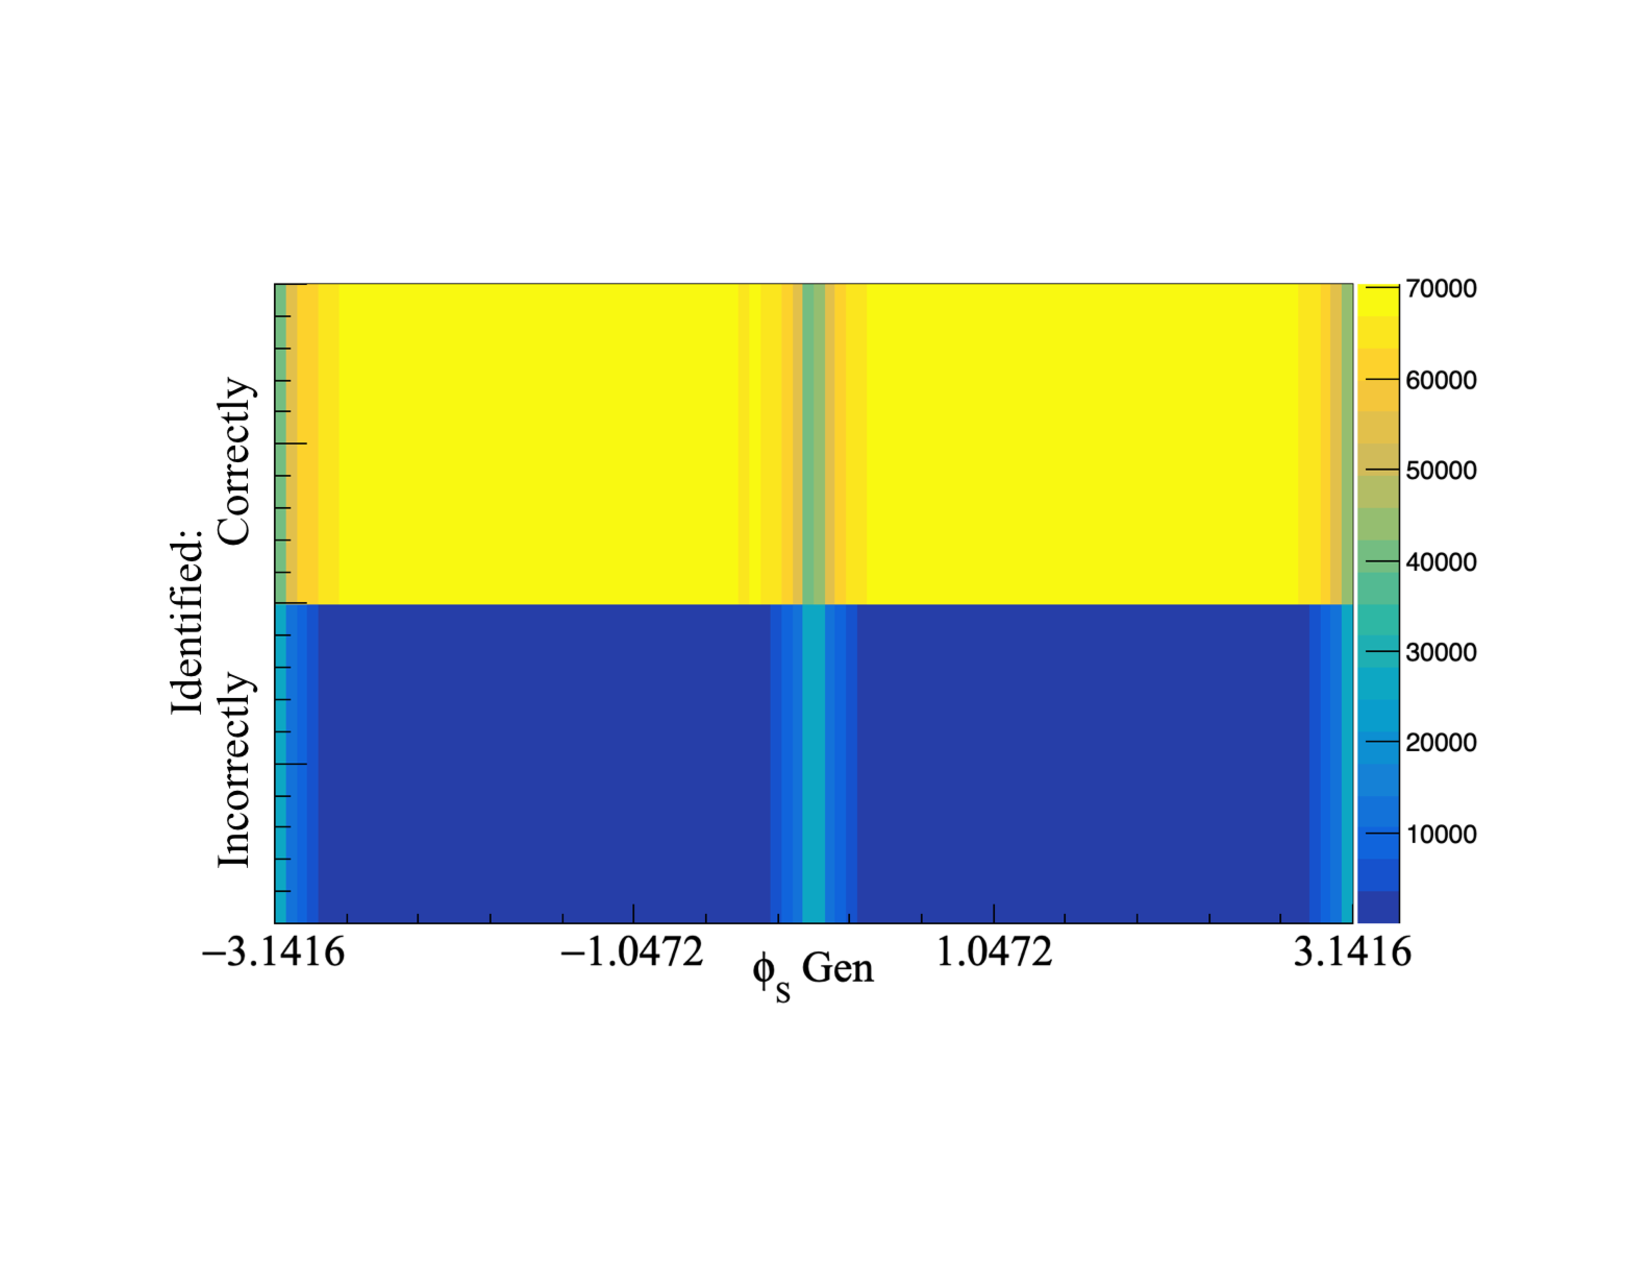
\includegraphics[width=\textwidth,trim=2cm 3cm 2cm 6cm, clip]{lrMigration}
  \caption{The rate of identified correctly and incorrectly left-right events as
    a function of $\phi_{\mathrm{S}}$.  This is determined by comparing the
    generated outgoing direction with the reconstructed outgoing direction.  The
    left-right boundary is clearing visible at 0$^{\circ}$ and -$\pi^{\circ}$
    and $\pi^{\circ}$}.
  \label{fig::lrMigration}
\end{figure}

\noindent
As is clearly visible there is a band of higher miss-identification rate at the
border between left and right.  For this reason a cut in the $\phi_{\mathrm{S}}$
variable symmetric about the left-right border was tested to determine the
percent of miss-identification as a function of the amount of
$\phi_{\mathrm{S}}$ cut.  These results are shown in
Fig.~\ref{fig::percentLRmiss}.

\begin{figure}[h!t]
  \centering
  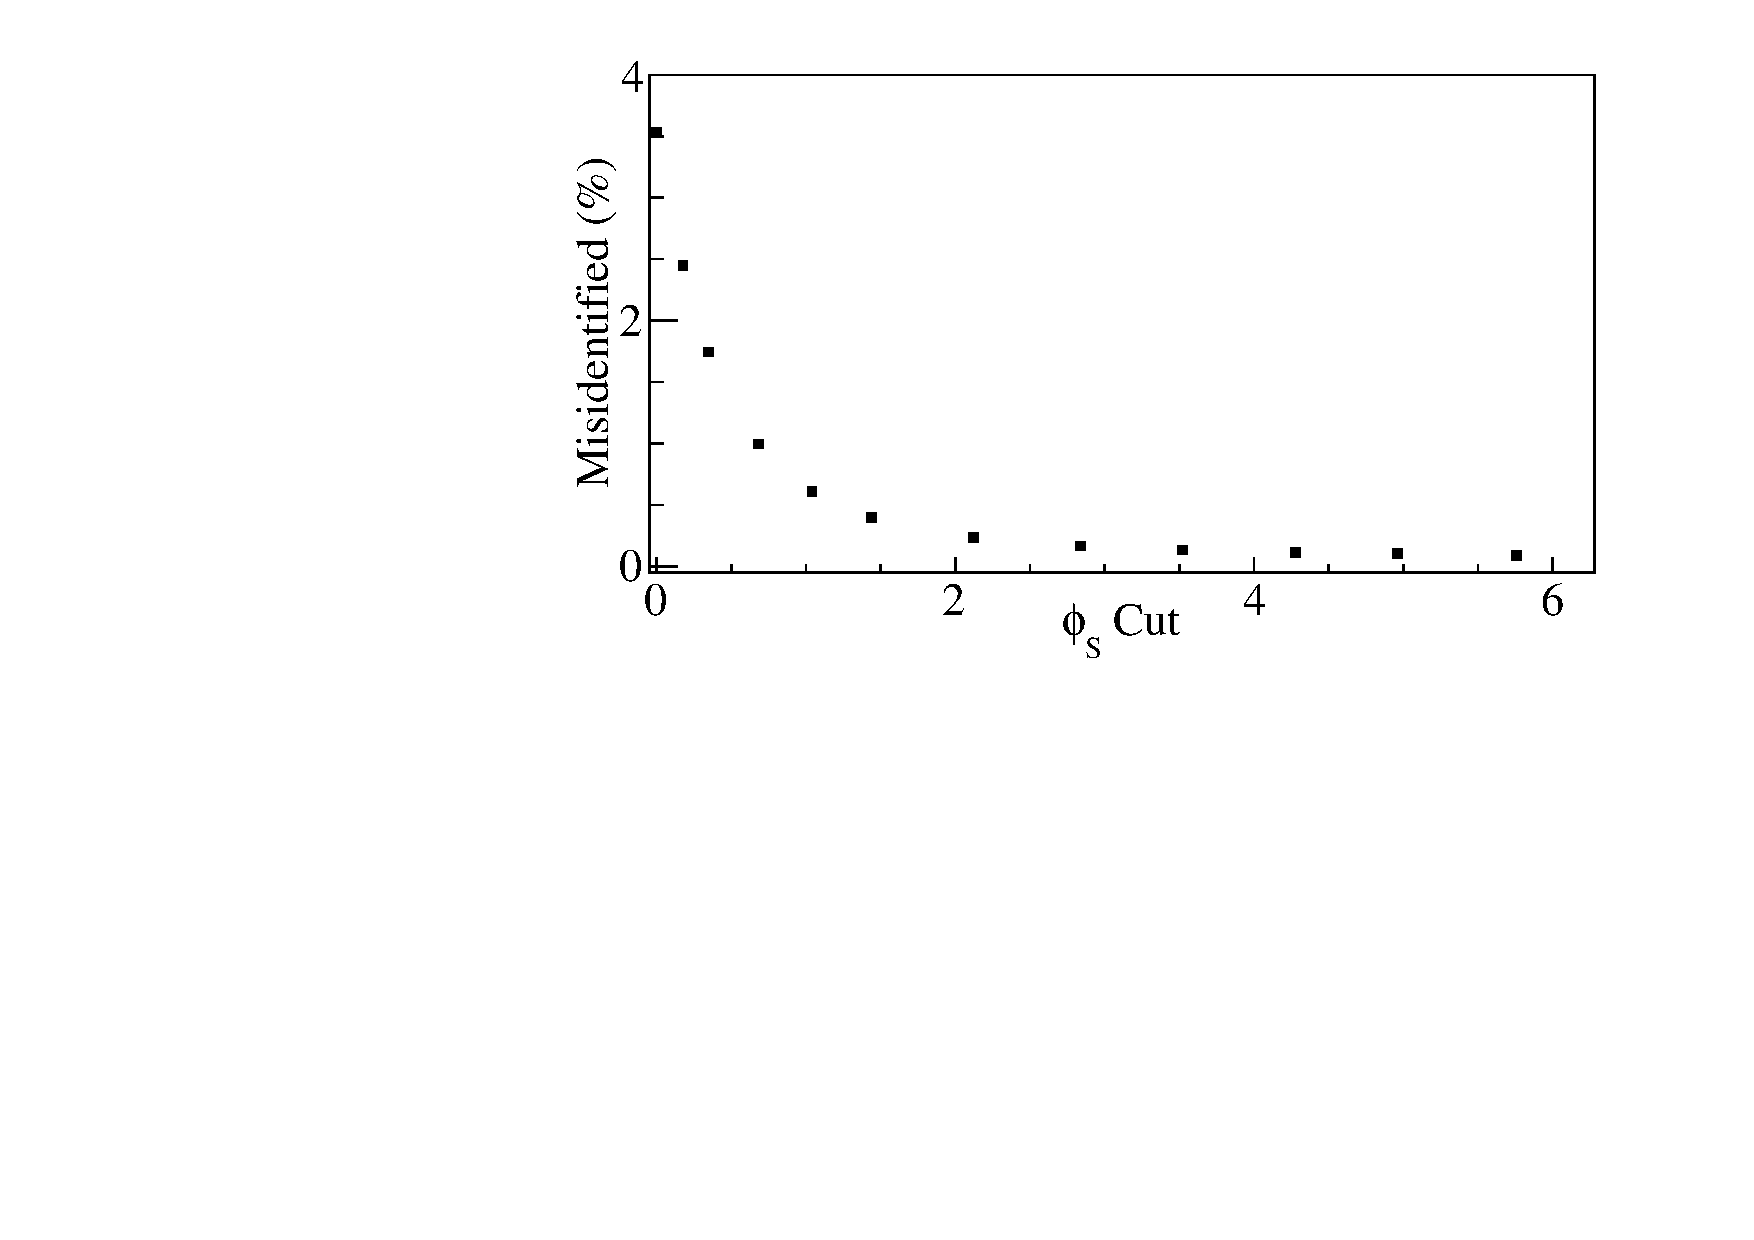
\includegraphics[width=0.8\textwidth]{percentLRmiss}
  \caption{Percent left-right migration as a function of the amount of
    $\phi_{\mathrm{S}}$ cut.}
    \label{fig::percentLRmiss}
\end{figure}

The systematic error for left-right migration is calculated as

\begin{equation}
  \delta \mathrm{A}_{\mathrm{N,systematic}} = \gamma *\mathrm{A}_{\mathrm{N}} +
  \gamma *\delta \mathrm{A}_{\mathrm{N}},
\end{equation}

\noindent
where this expression is derived in Appendix~\ref{app::sysLRmiss}.\par

No cut on $\phi_{\mathrm{S}}$ was used for the asymmetry due to the fact
that the systematic error is already small with no cut in $\phi_{\mathrm{S}}$
and to avoid loss of statistics.  The integrated systematic error due to
left-right event migration was determined to be 9\%.

\subsection{Total Systematics}
The total systematic error is determined by adding all non-zero systematic
effects in quadrature as

\begin{equation}
  \Big \langle
  \frac{
    \sigma_{\mathrm{systematics}}}{\sigma_{\mathrm{statistical}}}
  \Big \rangle =
  \sqrt{
    \sum_i^{\mathrm{all \; systematics}}
    \Big \langle
    \frac{\sigma^2_{\mathrm{systematics,
          i}}}{\sigma^2_{\mathrm{statistical}}}
    \Big \rangle
  } \;,
\end{equation}
where all the systematic effects considered are summarized in
Tab.~\ref{tab::sysError}.

\begin{table}[h!t]
  \centering
  \begin{tabular}{|c|c|c|c|}
    \hline
    \multirow{2}{*}{Systematic error}&
    \multirow{2}{*}{
      $\langle \sigma_{\mathrm{systematic}}/\sigma_{\mathrm{statistical}}
      \rangle$} &
    \multirow{2}{*}{$\langle \sigma_{\mathrm{systematic}} \rangle$} &
    \multirow{2}{*}{$\langle \sigma_{\mathrm{statistical}} \rangle$} \\
    
    & & & \\ \hline

    Period compatibility& 0.0 & 0.0 & 0.039\\ \hline

    Acceptance fluctuation& 0.2 & 0.008 & 0.039\\ \hline

    False asymmetry& 0.5 & 0.020 & 0.039\\ \hline

    Left-Right migration& 0.09 & 0.004 & 0.039\\ \hline

    Total& 0.55 & 0.021 & 0.039\\\hline
    
  \end{tabular}
  \caption{Summary of systematic error impacts to the integrated asymmetry}
  \label{tab::sysError}
\end{table}


\section{Results}
The asymmetries in this analysis are calculated from each of the separate nine
periods and then combined as a weighted average.  This calculation method is
used to minimize the effects of acceptance changes between periods as the
spectrometer was kept stable within each period but had the options for detector
changes and repairs between periods.  This resulting asymmetry for each method
is determined from a weighted average as
\begin{equation}
  \label{equ::wAvg}
  \mathrm{A}_{\mathrm{N}} = \sum_{\mathrm{period}}
  \frac{\mathrm{A}_{\mathrm{N},\mathrm{period}}\sigma^{-2}_{\mathrm{period}}}{\sigma^{-2}_{\mathrm{period}}},
  \quad \sigma^2 = \sum_{\mathrm{period}}
  \frac{1}{\sigma^{-2}_{\mathrm{period}}}.
\end{equation}

\noindent
The results for the basic geometric mean are shown in
Fig.~\ref{fig::ANgeom} and the results for the two target geometric mean
are shown in Fig.~\ref{fig::AN4TargGeom}.  The systematic error bars are
discussed in Sec.~\ref{sec::systematics}.

\begin{figure}[h!t]
  \begin{center}
    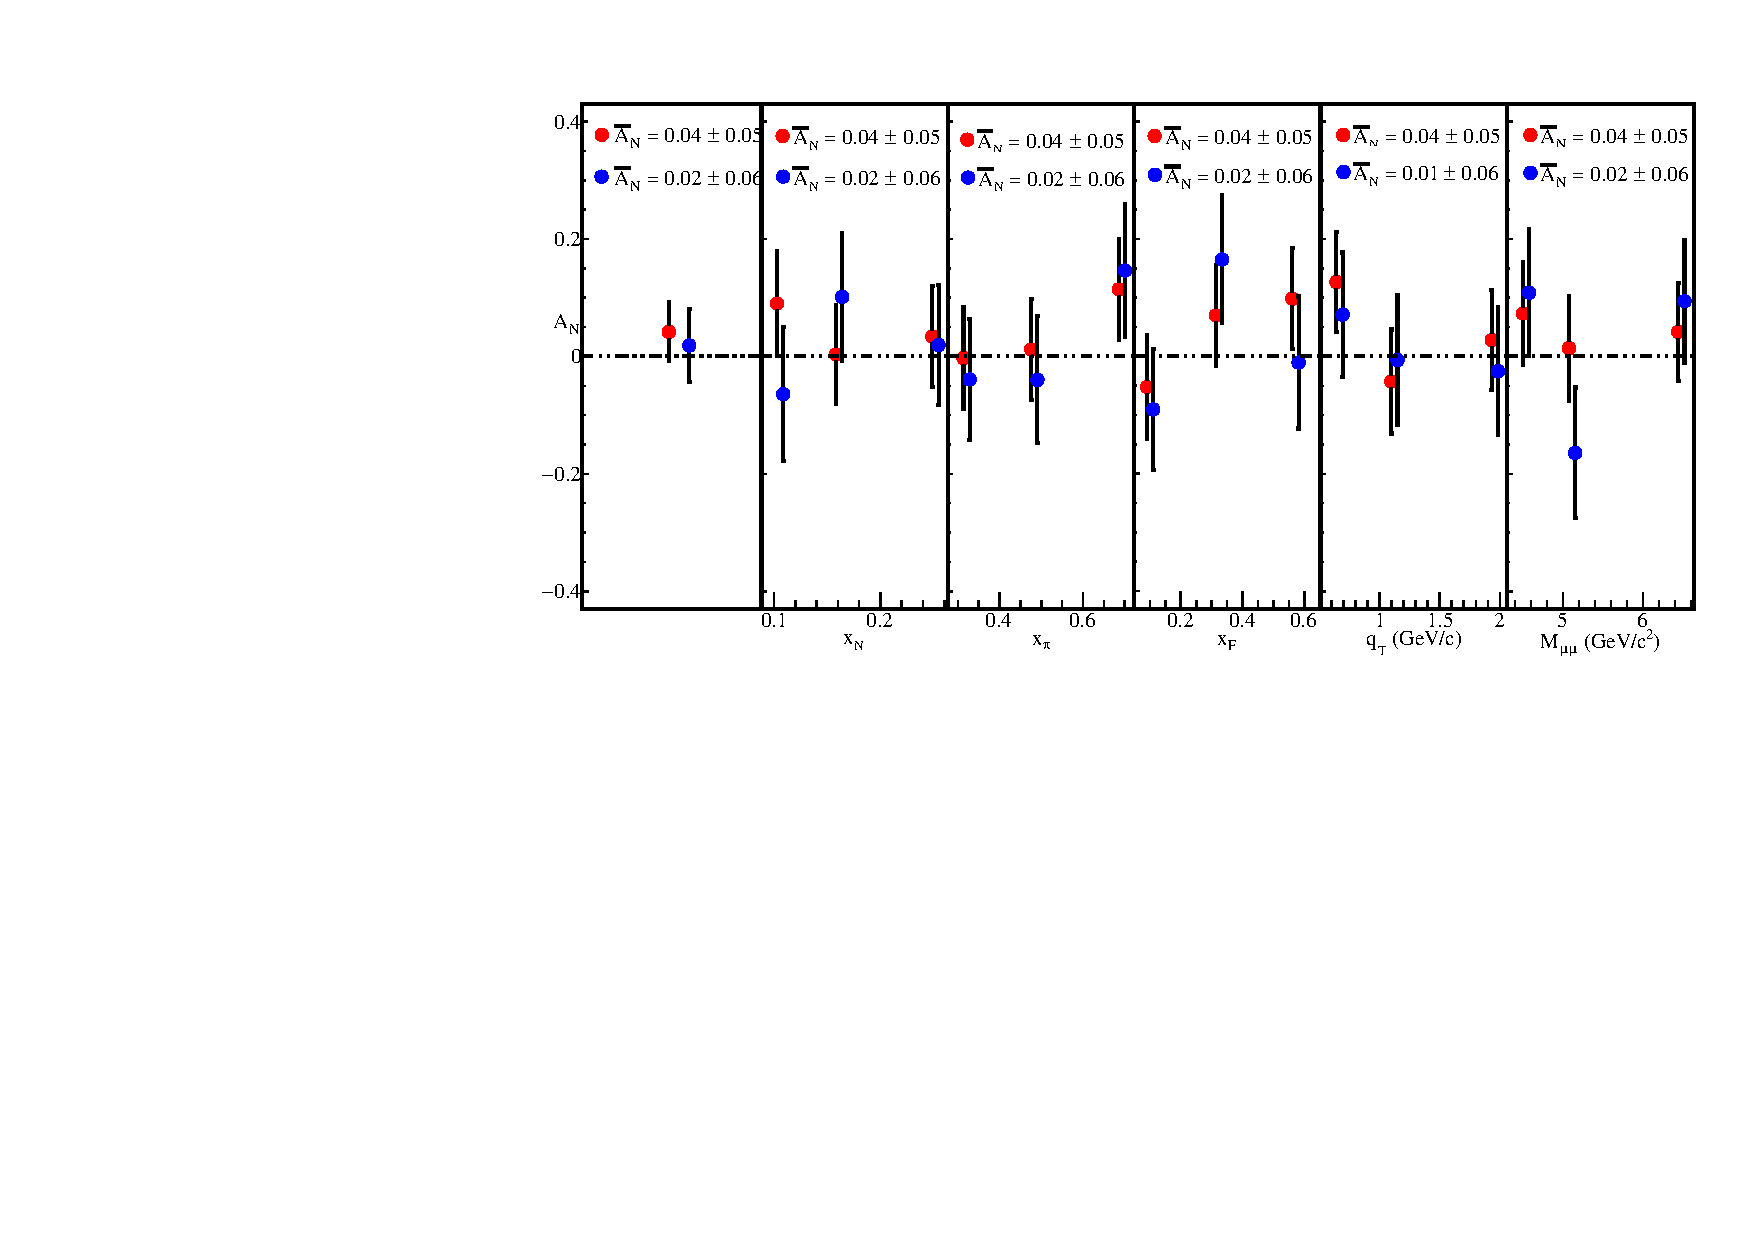
\includegraphics[width=\textwidth, trim=0.3cm 0cm 0.25cm 0cm, clip]{ANgeom} 
    \caption{A$_{\mathrm{N}}$ determined from the geometric mean method for the
      upstream target (red) and the downstream target (blue)}
    \label{fig::ANgeom}
  \end{center}
\end{figure}

\begin{figure}[h!t]
  \begin{center}
    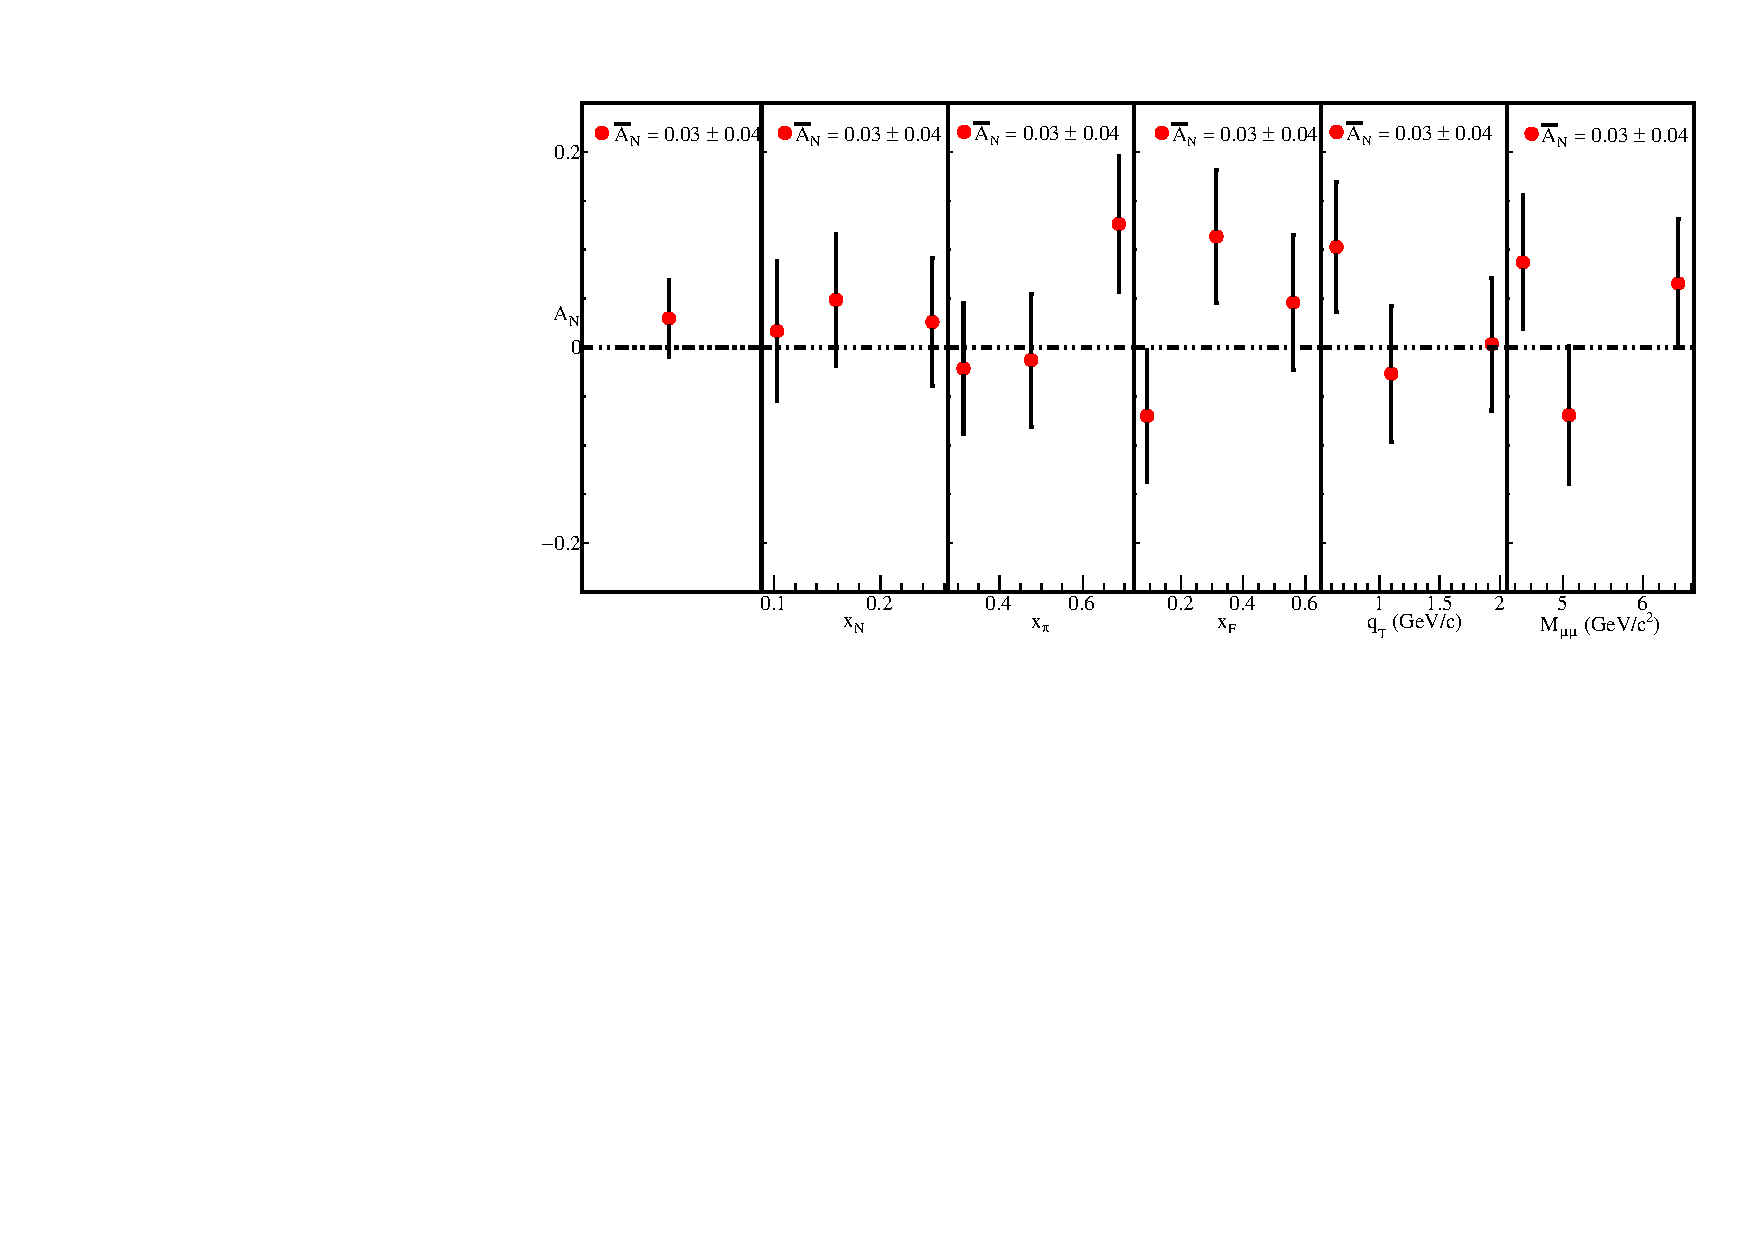
\includegraphics[width=\textwidth]{AN4TargGeom}
    \caption{A$_{\mathrm{N}}$ determined by the geometric mean method using both
      targets simultaneously}
    \label{fig::AN4TargGeom}
  \end{center}
\end{figure}

\subsection{Comparison of results}
